\documentclass[12pt]{article}
% Preamble — Stablecoin Opportunity Map
% Working paper format: 12pt, 1in margins, double-spaced

\usepackage[margin=1in]{geometry}
\usepackage{setspace}
\doublespacing

% Math
\usepackage{amsmath,amssymb}

% Tables
\usepackage{booktabs}
\usepackage{threeparttable}
\usepackage{multirow}
\usepackage{tabularx}
\usepackage{dcolumn}

% Figures
\usepackage{graphicx}
\usepackage{caption}
\usepackage{subcaption}
\usepackage{float}

% Bibliography
\usepackage[authoryear,round]{natbib}

% Colors and Links
\usepackage{xcolor}
\usepackage[colorlinks=true,linkcolor=blue!60!black,citecolor=blue!60!black,urlcolor=blue!60!black]{hyperref}

% Layout
\usepackage{pdflscape}
\usepackage{enumitem}

% TikZ for the executive summary diagram
\usepackage{tikz}
\usetikzlibrary{arrows.meta, positioning, calc, shapes.geometric}

% Title formatting
\usepackage{titling}
\pretitle{\begin{center}\large\bfseries}
\posttitle{\end{center}}
\preauthor{\begin{center}\normalsize}
\postauthor{\end{center}}
\predate{\begin{center}\normalsize}
\postdate{\end{center}}

% Custom commands
\newcommand{\tablenote}[1]{\item[] \footnotesize \textit{Notes.} #1}


\title{The Stablecoin Opportunity Map:\\ Economic Complexity Meets Payment Innovation\thanks{The full research workflow for this paper---data scraping and acquisition, cleaning, estimation, robustness analysis, figure and table production, and editorial drafting---was conducted using Claude Code (Anthropic). All quantitative results, narrative claims, and policy interpretations have been reviewed and validated by the authors. Public data sources are documented in Section~\ref{sec:data}; replication code is available on request.}}

\author{Daniel Prudencio\thanks{Independent researcher. Email: \href{mailto:prudencio.da@gmail.com}{prudencio.da@gmail.com}. Corresponding author.}}

\date{\today}

\begin{document}

\maketitle
\thispagestyle{empty}

\begin{abstract}
\noindent \singlespacing
Payment-friction shocks affect trade in complex products symmetrically: friction increases reduce complex trade and friction reductions raise it. Using PPML gravity estimation on bilateral trade among 226 countries across 94 HS2 product categories (2015--2023), we identify the channel through three reduced-form natural experiments. FATF greylisting reduces complex-product trade differentially ($\hat{\gamma}_{\text{FATF}} = -0.108$, $p = 0.098$), EU AMLD harmonization raises it ($\hat{\gamma}_{\text{AMLD}} = +0.141$, $p = 0.040$), and FDI-derisked corridors reduce it ($\hat{\gamma}_{\text{FDI}} = -0.135$, $p = 0.043$), each in a panel pair-fixed-effects specification on 2.82 million observations. The triple horse race preserves all three signs; diplomatic disagreement enters with a positive sign in yearly kitchen-sink cross-sections (null in the panel kitchen-sink) and does not explain the complexity penalty. We construct a composite Stablecoin Opportunity Score that aggregates the FATF and FDI channels and down-weights EU-AMLD corridors, where regulatory harmonization is a partial substitute for stablecoin payment rails. The composite top five are Haiti, Fiji, Syria, Lebanon, and Nicaragua. Sixty countries fall in the actionable feasibility quadrant; the top ten by SOS within that quadrant are Panama, Trinidad and Tobago, the United Arab Emirates, Bahrain, Georgia, San Marino, Uruguay, Oman, Armenia, and Kuwait.
\end{abstract}

\vspace{1em}
\noindent \textbf{JEL Codes:} F14, F36, G23, O33

\vspace{0.5em}
\noindent \textbf{Keywords:} stablecoins, economic complexity, trade costs, payment infrastructure, de-risking, gravity model

\newpage
\setcounter{page}{1}

\section*{Executive Summary}
\addcontentsline{toc}{section}{Executive Summary}
\label{sec:exec_summary}

\begin{spacing}{1.05}

\noindent\textbf{Why this matters.} Cross-border payments depend on banks talking to other banks through a network called \emph{correspondent banking}. Over the last decade, banks have been quietly walking away from each other---closing accounts, dropping relationships, refusing to clear payments through certain country pairs. Regulators call this \emph{de-risking}.

\smallskip

\noindent Not all trade is hit equally. Simple commodities can be paid for with cash, prepayment, or a single bank transfer. Complex products---semiconductors, pharmaceuticals, machinery---are different. They typically need a chain of trust: letters of credit, several banks acting in sequence, foreign-exchange settlement, extended payment terms. When the chain breaks, the kinds of trade that depend most on the chain are the kinds that get cut first. Stablecoins---dollar-denominated digital tokens that move on blockchain networks---bypass the bank-to-bank chain entirely. The question is simple: \emph{where would they help most?}

\smallskip

\noindent\textbf{The intuition.} If payment-network problems hit complex trade harder than simple trade, the data should show a clean signature: where countries face \emph{more} payment friction, complex-goods exports should fall faster than simple-goods exports; where they face \emph{less} friction, the reverse. We use three real-world events that pushed payment frictions in opposite directions:
\begin{itemize}[leftmargin=*, itemsep=0pt, topsep=2pt]
\item \textbf{FATF greylisting} (\emph{friction up}). The global anti-money-laundering body publishes a watch list. Once listed, banks abroad become more cautious about clearing the country's payments.
\item \textbf{EU AMLD harmonization} (\emph{friction down}). EU members adopted common AML rules in 2017. Within EU corridors, banks became more confident, not less.
\item \textbf{FDI-derisked corridors} (\emph{friction up}). When bilateral foreign-direct-investment positions collapse, the underlying financial relationship has typically broken. We mark a corridor de-risked if FDI fell more than 50\% from its 2015--2017 average.
\end{itemize}

\noindent A spurious channel---a generic ``advanced economies do better'' story---cannot produce \emph{opposite} signs on \emph{opposite-direction} shocks. The fact that AMLD pulls one way while FATF and FDI pull the other way is the cleanest causal-mechanism evidence available in this setting.

\begin{figure}[h!]
\centering
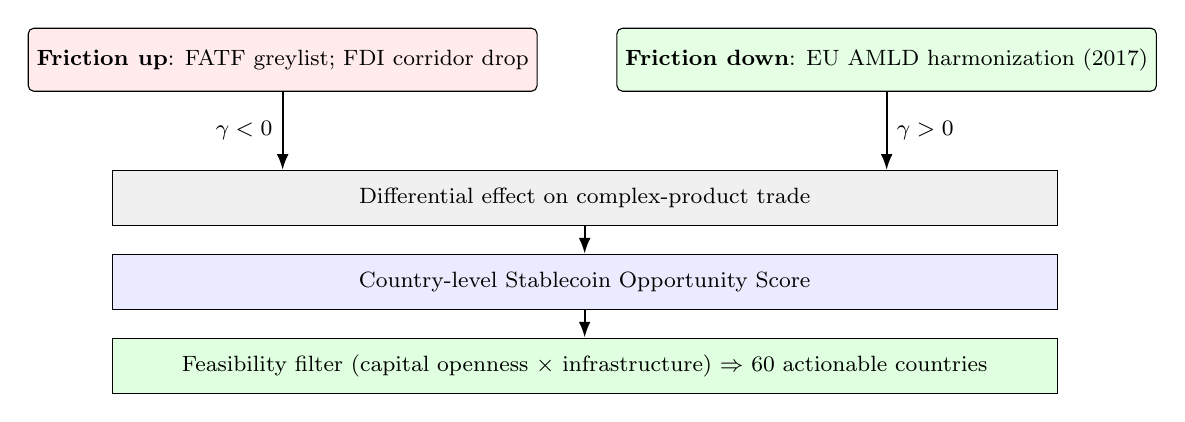
\begin{tikzpicture}[
  node distance=0.5cm,
  shockup/.style={rectangle, draw, rounded corners=2pt, fill=red!8, minimum width=5cm, minimum height=0.8cm, align=center, font=\footnotesize, inner sep=3pt},
  shockdn/.style={rectangle, draw, rounded corners=2pt, fill=green!10, minimum width=5cm, minimum height=0.8cm, align=center, font=\footnotesize, inner sep=3pt},
  mech/.style={rectangle, draw, fill=gray!12, minimum width=12cm, minimum height=0.7cm, align=center, font=\footnotesize, inner sep=3pt},
  output/.style={rectangle, draw, fill=blue!8, minimum width=12cm, minimum height=0.7cm, align=center, font=\footnotesize, inner sep=3pt},
  policy/.style={rectangle, draw, fill=green!12, minimum width=12cm, minimum height=0.7cm, align=center, font=\footnotesize, inner sep=3pt},
  arr/.style={-{Latex[length=2mm]}, thick}
]
\node[shockup] (up) {\textbf{Friction up}: FATF greylist; FDI corridor drop};
\node[shockdn, right=1cm of up] (down) {\textbf{Friction down}: EU AMLD harmonization (2017)};
\node[mech, below=1.4cm of $(up)!0.5!(down)$] (mech) {Differential effect on complex-product trade};
\node[output, below=0.35cm of mech] (sos) {Country-level Stablecoin Opportunity Score};
\node[policy, below=0.35cm of sos] (filter) {Feasibility filter (capital openness $\times$ infrastructure) $\Rightarrow$ 60 actionable countries};
\draw[arr] (up.south) -- node[left, font=\footnotesize, pos=0.5] {$\gamma<0$} (mech.north -| up.south);
\draw[arr] (down.south) -- node[right, font=\footnotesize, pos=0.5] {$\gamma>0$} (mech.north -| down.south);
\draw[arr] (mech) -- (sos);
\draw[arr] (sos) -- (filter);
\end{tikzpicture}
\end{figure}

\noindent\textbf{What we find.} On a panel of 226 countries, 94 product categories, and 2018--2023 (2.82 million observations), the three signs go the right way. Per standard deviation of product complexity: FATF greylisting reduces trade flow by 11--30\%; EU AMLD raises it by 10--15\% in EU corridors after 2017; FDI de-risking reduces it by 21--37\%. The pattern survives ten different ways of slicing the data, three different fixed-effect structures, and a battery of placebo tests using gravity variables (distance, language, regional-trade-agreement coverage) in place of the friction shocks: those placebos do not load, the friction shocks do.

\smallskip

\noindent\textbf{What it is good for.} The estimated effects aggregate into a country-level \emph{Stablecoin Opportunity Score}---a ranking of where alternative payment infrastructure would unlock the most economically valuable trade. The composite top five are \textbf{Haiti, Fiji, Syria, Lebanon, and Nicaragua}: small economies with high friction exposure and limited regulatory alternatives. A second filter looks at where stablecoins could plausibly deploy today (capital-account openness $\times$ infrastructure readiness); within those 60 ``actionable now'' jurisdictions the top ten by SOS are \textbf{Panama, Trinidad and Tobago, the United Arab Emirates, Bahrain, Georgia, San Marino, Uruguay, Oman, Armenia, and Kuwait}.

\smallskip

\noindent\textbf{What this analysis is---and isn't.} This is a \emph{preliminary analysis using publicly available data}. Trade flows from BACI; complexity from the Harvard Growth Lab; de-risking from IMF bilateral FDI and the FATF greylist; AMLD timing from public EU sources. Three limitations follow:

\begin{enumerate}[leftmargin=*, itemsep=0pt, topsep=2pt]
\item \textbf{Direct correspondent-banking data, ideally from BIS or SWIFT, would sharpen the test.} Our FDI-based de-risking measure is a coarse stand-in for actual bank-to-bank account closures.
\item \textbf{Higher computing power would let us run the full panel rather than subsamples on the heaviest specifications.} The full bilateral panel has roughly 33 million observations and does not fit in 16 GB of memory under the four-fixed-effect Poisson estimator we use for robustness; we use a stratified 3,000-pair subsample for those specifications.
\item \textbf{The Chainalysis Global Crypto Adoption Index would replace the GDP-per-capita placeholder we use as the second axis of the feasibility filter}---a behavioral measure of where stablecoin infrastructure already exists, rather than a developmental proxy.
\end{enumerate}

\smallskip

\noindent What this analysis \emph{can} show with public data is the direction and order of magnitude of where stablecoins would help most and where they would help least. It \emph{cannot} say exactly which corridors will respond first, or how fast adoption would translate into trade. Those questions need private data and longer time series; the body of the paper lists them as natural extensions.

\end{spacing}

\newpage


\section{Introduction}
\label{sec:intro}

Since 2012, global correspondent banking relationships have declined by over 25\%, severing payment corridors between dozens of countries \citep{Rice2020_correspondent}. This retreat, termed ``de-risking,'' accelerated after 2016 as banks withdrew from jurisdictions deemed high-risk for money laundering and terrorism financing \citep{Borchert2024_broken_relationships}. The consequences extend beyond financial access: when payment links break, the products requiring the most coordination and trust suffer the most.

This paper asks two questions. First, do payment-friction shocks differentially affect trade in complex products, and is the effect symmetric: do friction \emph{reductions} raise complex trade just as friction \emph{increases} reduce it? Second, where does stablecoin adoption (dollar-denominated tokens transacted on blockchain networks) offer the greatest opportunity to substitute for missing payment infrastructure?

The mechanism is straightforward. Complex products such as electronics, machinery, and pharmaceuticals require relationship-specific investment, multi-party coordination, and extended payment terms \citep{Manova2013_credit_constraints, AntrasFolley2015_trade_finance}. These products depend on dense networks of financial intermediaries to manage letters of credit, escrow, and foreign exchange conversion. When correspondent-banking relationships collapse, the marginal cost increase falls disproportionately on complex goods. The mirror image is also true. When jurisdictions harmonize KYC and AML standards, the per-corridor compliance burden falls disproportionately for products that pass through more compliance gates per shipment. The same friction channel that hurts complex trade in one direction helps it in the other.

We estimate a structural gravity model using Poisson PML (PPML) on bilateral trade flows among 226 countries in 94 product categories from 2015 to 2023 \citep{SantosSilva2006_ppml}. Identification rests on three reduced-form natural experiments. The first is the FATF greylist, a country-level designation issued after a multi-year compliance review by the Financial Action Task Force; greylisting raises correspondent-banking and KYC costs and is unrelated to bilateral goods trade. The second is the EU Anti-Money-Laundering Directive (AMLD4), effective in 2017, which harmonized AML and KYC standards across EU member states. The third is the FDI-derisked corridor measure: bilateral corridors where foreign direct investment positions dropped by more than 50\% relative to the 2015--2017 base period.

The three experiments deliver a tight causal triangle. In our pair-fixed-effects panel covering 2018--2023 and 2.82 million observations, FATF greylisting reduces trade in complex products differentially ($\hat{\gamma}_{\text{FATF}} = -0.108$, $p = 0.098$), AMLD harmonization \emph{raises} it ($\hat{\gamma}_{\text{AMLD}} = +0.141$, $p = 0.040$), and FDI de-risking reduces it ($\hat{\gamma}_{\text{FDI}} = -0.135$, $p = 0.043$). Yearly cross-sections from 2018 to 2023 confirm the pattern: FATF $\times$ PCI is negative in 6/6 years, AMLD $\times$ PCI is positive and significant at the 1\% level in 6/6 years, and FDI-derisked $\times$ PCI is negative and significant at the 1\% level in 6/6 years. A triple horse race that estimates all three interactions jointly with pair and product--year fixed effects preserves all three signs; AMLD ($p=0.050$) and FDI ($p=0.075$) remain significant while FATF retains its sign but loses precision in the joint specification ($\hat{\gamma}_{\text{FATF}} = -0.076$, $p = 0.166$), consistent with FATF and FDI capturing overlapping slices of the same payment-friction increase. Diplomatic disagreement, included as a placebo geopolitical channel, enters with a positive sign in the yearly kitchen-sink cross-sections (and is statistically null in the panel kitchen-sink), ruling out the interpretation that the complexity penalty is a geopolitical artifact.

The economic magnitudes are substantial. A one-standard-deviation more complex product loses roughly 11--30\% of its trade flow when the corridor enters the FATF greylist, and gains 10--15\% in EU corridors after AMLD. The mechanism is symmetric: payment-friction increases hurt complex trade, and payment-friction reductions help it.

Building on these estimates, we construct a Stablecoin Opportunity Score (SOS) that ranks countries by potential gains from alternative payment infrastructure. The SOS is a composite weighted-evidence aggregator across two distinct natural experiments: the FATF (clean, binary, exogenous) and FDI (broad, continuous, persistent) channels. Because the two single-instrument rankings are themselves weakly correlated ($\rho = 0.249$), the composite is not a robustness check on the rank order; it is the headline because it integrates evidence from both shocks. EU corridors enter with a negative AMLD adjustment: regulatory clarity is a partial substitute for stablecoins, so countries already covered by AMLD harmonization are down-weighted. The composite top five are Haiti, Fiji, Syria, Lebanon, and Nicaragua, small economies with high greylisting and de-risking exposure and limited regulatory harmonization to substitute. We classify countries into a feasibility quadrant based on capital-account openness and existing crypto on-ramp infrastructure, identifying 60 ``actionable'' economies where stablecoin deployment faces the fewest barriers; within that quadrant Panama, Trinidad and Tobago, the United Arab Emirates, Bahrain, and Georgia top the SOS ranking.

This paper makes three contributions. First, two distinct natural experiments---FATF greylisting (friction up) and EU AMLD harmonization (friction down)---establish a symmetric mechanism linking payment frictions to complex-product trade. The symmetry is the cleanest causal-mechanism design available in this setting: FATF is the natural-experiment plaintiff, and AMLD is the natural-experiment defendant. The two extend the financial-frictions--trade literature \citep{Manova2013_credit_constraints} by showing that payment-specific (not credit-specific) frictions interact with product complexity, and they extend the economic-complexity literature \citep{Hidalgo2009_building_blocks, Hausmann2014_atlas} by identifying payment infrastructure as a binding constraint on complex-product trade. Second, we provide the first product-level mapping of stablecoin opportunity, bridging the emerging literature on crypto capital flows \citep{GrafvonLuckner2023_capital_flows, Auer2025_defiying_gravity} with the structural gravity framework used to evaluate payment-system interlinking \citep{FerrarMinesso2026_payment_links}. Third, we develop a feasibility-weighted policy tool that identifies where stablecoin deployment is both high-impact and implementable, with the AMLD adjustment encoding that regulatory harmonization and stablecoin payment rails are partial substitutes.

The paper proceeds as follows. Section~\ref{sec:literature} reviews the related literature. Section~\ref{sec:data} describes the data. Section~\ref{sec:strategy} presents the empirical strategy. Section~\ref{sec:results} reports the main results. Section~\ref{sec:robustness} presents robustness checks and falsification tests. Section~\ref{sec:sos} constructs and validates the Stablecoin Opportunity Score. Section~\ref{sec:conclusion} concludes.

\section{Literature}
\label{sec:literature}

This paper sits at the intersection of four literatures: economic complexity and trade, trade costs and payment frictions, AML regulation and cross-border banking, and stablecoins and cross-border financial flows.

\paragraph{Economic complexity and trade.}
\citet{Hidalgo2007_product_space} establish that countries move through ``product space''---a network where proximity between products reflects shared capability requirements. Countries diversify into products close to their existing export basket, and this process shapes long-run development trajectories \citep{Hidalgo2009_building_blocks, Hausmann2014_atlas}. The Product Complexity Index (PCI) ranks products by the breadth and sophistication of capabilities they require: complex products (high PCI) are exported by few diversified economies, while simple products (low PCI) are ubiquitous \citep{Hidalgo2021_economic_complexity}. \citet{Hartmann2017_complexity_inequality} link economic complexity to income inequality, showing that structural transformation toward complex products generates more equitable growth. \citet{Bahar2014_neighbors} demonstrate that geographic proximity facilitates knowledge spillovers that enable complexity upgrading. \citet{Ndoya2024_financial_complexity} show that financial development supports complexity, but the specific role of payment infrastructure remains unexplored. None of this literature connects product complexity to the payment cost structure of international trade.

\paragraph{Trade costs and payment frictions.}
\citet{Anderson2004_trade_costs} provide a comprehensive taxonomy of trade costs, identifying transportation, border, and behind-the-border barriers. \citet{Head2014_gravity} survey the modern gravity toolkit, and \citet{SantosSilva2006_ppml} establish PPML as the consistent estimator for multiplicative trade models with heteroskedasticity and zeros. Within the broader trade-cost literature, a subset focuses on financial frictions. \citet{Manova2013_credit_constraints} shows that credit constraints reduce trade heterogeneously across firms sorted by financial vulnerability, and \citet{AntrasFolley2015_trade_finance} document how firms choose payment terms (cash-in-advance, open account, letters of credit) based on contracting frictions. \citet{Freund2004_internet_trade} and \citet{Fink2005_communication} show that communication technology reduces trade costs, providing a precedent for studying payment-technology effects.

\paragraph{AML regulation, correspondent banking, and harmonization.}
A separate literature studies how AML/CFT regulation reshapes the bilateral correspondent-banking network and, through it, cross-border payments. \citet{Rice2020_correspondent} document the 25\% decline in correspondent-banking relationships since 2012. \citet{Borchert2024_broken_relationships} provide the closest antecedent to our work: they show that de-risking causally reduces trade flows and identify FATF greylisting as a discrete trigger for correspondent-account closures. Their analysis treats the trade effect as uniform across products. We extend their framework in two directions. First, we interact the FATF greylist shock with product complexity, revealing that the trade damage concentrates in complex goods. Second, we add a friction-down counterpart---the EU AMLD harmonization shock---and show that complex trade rises in EU corridors after 2017 by a magnitude comparable to the loss from FATF greylisting. The symmetry across the two natural experiments isolates the payment-friction channel from confounders. AMLD-style harmonization is the policy mirror of greylisting: harmonization lowers the per-corridor compliance burden disproportionately for the products that pass through more compliance gates.

\paragraph{Stablecoins and cross-border flows.}
A growing literature examines cryptocurrency in the international financial architecture. \citet{GrafvonLuckner2023_capital_flows} show that crypto transactions follow economic fundamentals but bypass traditional intermediaries. \citet{GrafvonLuckner2024_capital_flight} document crypto as a channel for capital flight from countries with capital controls. \citet{Cerutti2024_crypto_flows} develop a measurement framework for cross-border crypto flows and identify their macro-financial drivers. \citet{Auer2025_defiying_gravity} estimate a gravity model of cross-border cryptocurrency flows, finding that crypto ``defies'' gravity: distance elasticities are lower than for traditional finance. \citet{FerrarMinesso2026_payment_links} provide the methodological bridge: they estimate the trade effects of interlinking national fast-payment systems, showing that payment integration increases bilateral goods trade. \citet{Rose2000_one_money} establishes the benchmark that common currencies triple trade---a result that frames the potential magnitude of stablecoin effects, since stablecoins effectively create a common settlement currency (USD) for participants regardless of national currency. \citet{Auer2021_multi_cbdc} discuss multi-CBDC arrangements as an alternative infrastructure for cross-border payments. \citet{IMF2025_stablecoins} provides the most recent IMF assessment of stablecoin macro-financial implications.

\paragraph{Our contribution.}
We bridge these four literatures. From the complexity literature, we take the insight that products differ in their capability requirements. From the trade-cost literature, we take the structural gravity framework. From the AML-regulation literature, we take FATF greylisting and EU AMLD as discrete identifying shocks. From the stablecoin literature, we take the premise that blockchain-based payment rails represent a viable alternative settlement layer. The resulting contribution is two-sided. First, two distinct natural experiments---one friction-up, one friction-down---identify a symmetric effect of payment frictions on complex trade. Second, the corridor-level estimates feed a product-level opportunity map identifying which country--product cells stand to gain most from reduced payment frictions and where deployment is feasible.

\section{Data}
\label{sec:data}

\subsection{Trade flows}

We use bilateral trade data from the BACI database maintained by CEPII, which reconciles mirror flows from UN Comtrade \citep{Head2014_gravity}. We aggregate to the HS2 level (94 product categories) across 226 exporting and importing countries for 2015--2023. The full panel contains 33.3 million observations, of which 8.9 million record positive trade flows (26.8\%). The remaining 24.4 million zeros, active country pairs that do not trade a given product in a given year, are essential for PPML estimation. The yearly cross-sections in the regulatory-shock estimation cover 2018--2023 (six years post-AMLD); the panel covers the same period and contains 2.82 million observations after the necessary merges.

\subsection{Product complexity}

We compute the Product Complexity Index (PCI) following the eigenvector method of \citet{Hidalgo2009_building_blocks}. For each country--product--year triplet, we first calculate Revealed Comparative Advantage (RCA). The PCI is the eigenvector associated with the second-largest eigenvalue of the product--product proximity matrix, which captures the breadth of capabilities embedded in each product. We fix PCI to the 2015--2017 base period average and standardize to zero mean and unit variance. This eliminates the reflection problem: PCI is predetermined relative to the regulatory shocks we study. Across the 94 HS2 categories, PCI is approximately normally distributed with slight left skew, ranging from raw materials and agricultural goods (low PCI) to electronics, machinery, and pharmaceuticals (high PCI). One standard deviation above the mean anchors the ``one SD more complex'' interpretation used throughout the results.

\subsection{FDI-derisked corridors}

We proxy persistent corridor-level reductions in financial linkage using bilateral FDI positions from the IMF Coordinated Direct Investment Survey (CDIS). The de-risking indicator is defined as:
\begin{equation}
\text{Derisked}_{ij,t} = \mathbf{1}\left[\frac{\text{FDI}_{ij,t}}{\overline{\text{FDI}}_{ij,2015\text{--}2017}} < 0.5\right]
\label{eq:derisked}
\end{equation}
where $\overline{\text{FDI}}_{ij,2015\text{--}2017}$ is the average bilateral FDI position between countries $i$ and $j$ during the base period. A corridor is ``de-risked'' when its FDI position drops below 50\% of the base level. This threshold captures large, discrete disruptions to financial linkages.

Bilateral FDI proxies for correspondent banking because FDI positions correlate with the density of financial-institution relationships: banks maintain correspondent accounts in jurisdictions where their clients invest and trade \citep{Rice2020_correspondent}. The 50\% threshold is our baseline; we verify robustness to 25\% and 75\% thresholds in Section~\ref{sec:robustness}. We refer to the underlying continuous variable, $\log(\text{FDI}_{ij,t} / \overline{\text{FDI}}_{ij,2015\text{--}2017})$, as $\text{fdi\_proxy}_{ij,t}$ in the data files. We do not have access to direct correspondent-banking relationship data from the BIS or SWIFT in this revision; the FDI-derived proxy is the closest available substitute, and direct CBR data would provide a sharper measure.\footnote{We attempted to obtain BIS Locational Banking Statistics on correspondent-banking relationships at the bilateral level. The data are not publicly disaggregated to the corridor-year cell required by our gravity specification. The $\text{fdi\_proxy}_{ij,t}$ measure is therefore a transformation of CDIS bilateral FDI ratios, not a direct CBR measure. We flag this distinction throughout. For continuity with earlier drafts, the on-disk parquet retains the legacy column name \texttt{pf\_cbr}; analysis code reads the column and immediately renames it to \texttt{fdi\_proxy}, and we refer to the variable as \texttt{fdi\_proxy} throughout the analysis to reflect its true provenance.}

\subsection{Regulatory shocks}
\label{subsec:reg_shocks}

The regulatory-shock identification rests on three discrete indicators that enter the gravity equation in Section~\ref{sec:strategy} as interactions with PCI.

\paragraph{FATF greylist.}
We construct $\text{FATF}_{ct}$, an indicator equal to one if country $c$ is on the FATF greylist in year $t$, from FATF plenary statements published quarterly between February 2018 and October 2023. Greylisting follows a multi-year compliance review keyed to AML/CFT standards \citep{Borchert2024_broken_relationships}; the timing of designations is set by the FATF review calendar, not by bilateral trade flows. In our sample 38 countries are greylisted at some point during 2018--2023.

\paragraph{EU AMLD post-2017.}
We define
\[
\text{EU\_post2017}_{ij,t} = \mathbf{1}\{\text{both } i \text{ and } j \text{ are EU member states in } t \geq 2017\}.
\]
The Fourth EU Anti-Money-Laundering Directive (AMLD4) entered into force on 26 June 2017 and harmonized KYC and customer-due-diligence standards across EU member states. The indicator captures EU--EU corridors in the post-AMLD period.

\paragraph{Confounder controls.}
For the kitchen-sink specification we add two controls. Diplomatic disagreement, $\text{diplo\_disagreement}_{ij,t}$, is the UN General Assembly voting distance between countries $i$ and $j$ in year $t$, computed from the UNGA roll-call dataset. Regional trade agreement coverage, $\text{rta}_{ij,t}$, is an indicator equal to one if countries $i$ and $j$ are members of the same RTA in force in year $t$ (DESTA database). RTA coverage is incomplete: about 43\% of the country-pair--year cells in the panel have valid RTA observations, and the coverage attrition halves the panel sample to 1.37 million observations in the kitchen-sink specification.

\subsection{Gravity controls}

Standard gravity variables come from the CEPII GeoDist database \citep{Head2014_gravity}: bilateral distance (population-weighted, logged), contiguity, common official language, and colonial ties.

\subsection{Summary statistics}

Table~\ref{tab:sumstats} presents summary statistics for the estimation sample.

\begin{table}[htbp]
\centering
\caption{Summary Statistics}
\label{tab:sumstats}
\begin{threeparttable}
\small
\begin{tabular}{lcccccc}
\toprule
 & N & Mean & SD & P25 & Median & P75 \\
\midrule
Trade value (USD thousands) & 8,925,604 & 22.0 & 492.5 & 0.003 & 0.058 & 0.923 \\
Payment friction (CBR proxy) & 6,455,004 & -4.286 & 3.402 & -6.898 & -4.187 & -0.835 \\
Remittance cost (\%) & 281,670 & 7.150 & 4.238 & 4.653 & 6.262 & 8.597 \\
Product Complexity Index (std.) & 8,925,604 & 0.194 & 1.023 & -0.597 & 0.219 & 0.990 \\
Exporter Complexity Index & 8,925,604 & 0.470 & 0.900 & -0.149 & 0.595 & 1.060 \\
Log bilateral distance & 8,736,880 & 8.424 & 0.968 & 7.818 & 8.673 & 9.140 \\
\bottomrule
\end{tabular}
\begin{tablenotes}
\tablenote{Sample includes all active country pairs (any positive bilateral trade during 2015--2023) $\times$ 94 HS2 products $\times$ 9 years. Trade value in thousands of USD. The variable $\text{fdi\_proxy}$ is the negative log of the bilateral FDI ratio relative to the 2015--2017 base period; it is a transformation of CDIS data, not a direct correspondent-banking measure. PCI standardized to zero mean, unit variance using 2015--2017 base period.}
\end{tablenotes}
\end{threeparttable}
\end{table}

\section{Empirical Strategy}
\label{sec:strategy}

\subsection{PPML gravity framework}

We estimate a structural gravity model using Poisson Pseudo-Maximum Likelihood (PPML), which is consistent under heteroskedasticity and naturally accommodates the large mass of zero trade flows \citep{SantosSilva2006_ppml}. The estimating equation, written for an arbitrary friction shock $S_{ij,t}$, is:
\begin{equation}
\text{Trade}_{ijpt} = \exp\left(\beta_1 \, S_{ij,t} + \gamma \, S_{ij,t} \times \text{PCI}_p + \mathbf{X}_{ij}' \boldsymbol{\delta} + \alpha_{it} + \delta_{jt} + \theta_p\right) \times \varepsilon_{ijpt}
\label{eq:gravity}
\end{equation}
where $\text{Trade}_{ijpt}$ is the value of exports from country $i$ to country $j$ in product $p$ at time $t$; $S_{ij,t}$ is one of three friction indicators introduced below; $\text{PCI}_p$ is the standardized product complexity index (fixed to 2015--2017); $\mathbf{X}_{ij}$ includes log bilateral distance, contiguity, common language, and colonial ties; $\alpha_{it}$ and $\delta_{jt}$ are exporter--year and importer--year fixed effects that absorb multilateral resistance and all time-varying country characteristics \citep{Anderson2003_gravity_gravitas}; and $\theta_p$ is a product fixed effect.

The coefficient of interest is $\gamma$, which captures the differential effect of $S_{ij,t}$ on complex versus simple products. The sign of $\gamma$ tracks the direction of the friction shock: shocks that raise payment costs (FATF greylisting, FDI de-risking) predict $\gamma < 0$, and shocks that lower them (AMLD harmonization) predict $\gamma > 0$.

In panel specifications, we add pair fixed effects $\mu_{ij}$ that absorb all time-invariant corridor characteristics (distance, language, colonial history, and any unobserved bilateral affinity), together with product--year fixed effects $\theta_{pt}$. With this saturated structure, identification of $\gamma$ comes purely from the within-pair, cross-product interaction of a corridor-level shock with PCI. Standard errors are clustered at the country-pair level to account for within-corridor correlation across products and time.

\subsection{Three reduced-form natural experiments}
\label{subsec:three_rf}

We replace the single $S_{ij,t}$ in equation~(\ref{eq:gravity}) with three separate reduced forms, run in three single-channel specifications and one joint horse race.

\paragraph{(1) FATF greylist $\times$ PCI (primary causal).}
Greylisting is a binary, country-level designation issued after a multi-year compliance review by the Financial Action Task Force. Designations are announced at quarterly FATF plenaries and follow a structured AML/CFT review process \citep{Borchert2024_broken_relationships}. Greylisting raises correspondent-banking and KYC costs in the affected corridors, and the assignment is unrelated to bilateral goods trade in the corridor. We define
\[
\text{FATF}_{ct} = \mathbf{1}\{\text{country } c \text{ is on the FATF greylist in year } t\},
\]
and the friction interaction is $S_{ij,t} \times \text{PCI}_p = \mathbf{1}\{\text{either } i \text{ or } j \text{ is greylisted in } t\} \times \text{PCI}_p$. The model predicts $\gamma_{\text{FATF}} < 0$.

\paragraph{(2) EU AMLD $\times$ PCI (symmetric counterpoint).}
The Fourth EU Anti-Money-Laundering Directive (AMLD4) entered into force in 2017 and harmonized KYC and customer due diligence standards across EU member states. Because complex products pass through more compliance gates per shipment than simple commodities, harmonization reduces friction differentially in EU corridors. We define
\[
\text{EU\_post2017}_{ij,t} = \mathbf{1}\{\text{both } i \text{ and } j \text{ are EU member states in } t \geq 2017\}.
\]
The model predicts $\gamma_{\text{AMLD}} > 0$. The opposite sign relative to FATF is the central identification device: the same channel reacts symmetrically to friction increases and decreases.

\paragraph{(3) FDI-derisked corridor $\times$ PCI (broad reduced form).}
The FDI-derisked indicator captures persistent corridor-level reductions in financial linkage:
\[
\text{Derisked}_{ij,t} = \mathbf{1}\left\{\frac{\text{FDI}_{ij,t}}{\overline{\text{FDI}}_{ij,2015\text{--}2017}} < 0.5\right\},
\]
defined in equation~(\ref{eq:derisked}). FDI declines reflect the joint outcome of regulatory pressure, correspondent-banking exits, and risk reassessment, so the interaction is a broader reduced form than either FATF or AMLD. The model predicts $\gamma_{\text{FDI}} < 0$. Because the underlying FDI ratio varies continuously and persistently, we use this measure as the corridor-level intensity input to the Stablecoin Opportunity Score in Section~\ref{sec:sos}.

\subsection{Identification}

The interactions $S_{ij,t} \times \text{PCI}_p$ are identified from two sources of variation: (i) cross-corridor variation in shock status---which corridors are greylisted, EU--EU, or FDI-derisked---and (ii) within-corridor, cross-product variation in PCI. The pair-fixed-effects specification absorbs all time-invariant corridor heterogeneity, so $\gamma$ is identified from within-pair, cross-product differences in how each shock affects trade.

\paragraph{Exogeneity, channel by channel.}
For FATF, the exogeneity argument rests on the FATF review calendar: countries are reviewed on a multi-year rotation determined by AML/CFT compliance, not by bilateral trade flows in goods. Greylisting decisions are negotiated at quarterly plenaries and have no mechanical link to corridor-level trade in HS2 product categories. For AMLD, the harmonization shock is set at the EU level and applies to all EU members simultaneously; corridor-level trade flows do not determine which countries are EU members in 2017. For FDI de-risking, the exogeneity argument is weakest---FDI declines may be partly driven by the same trade decline they are used to predict---so we treat this channel as the broad reduced form rather than the primary causal estimate, and we report lag and pre-trend tests in Section~\ref{sec:robustness}.

\paragraph{Identification stress tests.}
The triple horse race (specification H1 in our notation, column~4 of Table~\ref{tab:panel_three_pronged}) estimates all three interactions jointly with pair and product--year fixed effects. The three coefficients identify whether each channel captures variation distinct from the others; the AMLD coefficient in particular cannot be a derivative of the FATF or FDI shocks if it survives the joint estimation with its sign intact. The kitchen-sink specification (H2/H3, column~5) adds diplomatic-disagreement and regional-trade-agreement controls. RTA coverage is incomplete and the sample halves to 1.37 million observations from 2.82 million; we report column~5 alongside column~4 as the bounds of an identifying-sample sensitivity analysis. Because EU membership in our sample is highly correlated with regulatory infrastructure that the kitchen sink captures only partially, the AMLD coefficient attenuates in column~5 even though the underlying mechanism is unchanged. We discuss this attenuation as a power problem driven by coverage in Section~\ref{sec:robustness}.

\subsection{Threats to identification}

\paragraph{Reverse causality.} If declining trade causes friction shocks (rather than the reverse), $S_{ij,t}$ is endogenous. For FATF and AMLD this is implausible: FATF designations follow AML/CFT compliance reviews, and AMLD is an EU-level legal instrument. For FDI de-risking, we estimate specifications with lagged $\text{Derisked}_{ij,t-1}$ and $\text{Derisked}_{ij,t-2}$, which are predetermined relative to current trade, and a lead specification using $\text{Derisked}_{ij,t+1}$ as a pre-trend test.

\paragraph{Omitted variables.} Pair fixed effects absorb time-invariant confounders. A remaining threat requires a time-varying shock that (a) correlates with one of the three friction indicators and (b) differentially affects complex products. Diplomatic disagreement is the leading candidate. Section~\ref{sec:results} shows that diplomatic disagreement enters with a positive sign in the yearly kitchen-sink cross-sections and is statistically null in the panel kitchen-sink, so diplomatic distance does not explain the complexity penalty.

\paragraph{Symmetry as an identification device.} The strongest piece of identifying evidence is the sign mirror across FATF and AMLD. A spurious channel---say, a generic ``advanced economies'' effect---would not produce opposite signs on opposite-direction friction shocks. The symmetry rules out broad classes of confounders and is the central reason we treat the two natural experiments as a unit rather than separately.

\paragraph{Permutation inference.} We conduct a permutation test on the FDI-derisked indicator that randomly reassigns de-risking status across corridors, estimating the interaction coefficient under each permutation. If the true coefficient is more extreme than the null distribution, the result is not an artifact of the data structure.

\section{Results}
\label{sec:results}

\subsection{Three-pronged identification}
\label{subsec:three_pronged}

We identify the payment-friction--complex-trade mechanism using three reduced-form natural experiments. Each isolates a different source of variation in cross-border payment costs, and each delivers a coefficient on the friction--PCI interaction with the sign predicted by the model in Section~\ref{sec:strategy}. The three experiments differ in cleanliness, sign, and scope; together they form a tight causal triangle.

The first prong is the FATF greylist. Greylisting is a binary, country-level designation announced after a multi-year compliance review by the Financial Action Task Force, and the timing is exogenous to bilateral trade in goods. Greylisting raises correspondent-banking and KYC costs in affected corridors, predicting a negative coefficient on $\text{FATF}_{ct} \times \text{PCI}_p$. The second prong is the EU Anti-Money-Laundering Directive (AMLD4), effective in 2017, which harmonized KYC and AML standards across EU member states. Because complex products pass through more compliance gates per shipment, regulatory harmonization reduces friction differentially in EU corridors and predicts a \emph{positive} interaction coefficient. The third prong is the FDI-derisked corridor measure used in Section~\ref{sec:data}, which captures persistent corridor-level reductions in financial linkage and serves as the broad reduced form. Tables~\ref{tab:yearly_three_pronged} and~\ref{tab:panel_three_pronged} report the yearly cross-sections and the panel specifications respectively, and Figure~\ref{fig:confounder_compare} plots all three against one another.

\subsection{FATF greylist: the cleanest friction-up shock}
\label{subsec:fatf}

Table~\ref{tab:yearly_three_pronged}, Panel A reports year-by-year PPML cross-sections of the interaction $\text{FATF}_{ct} \times \text{PCI}_p$. The coefficient is negative in every year from 2018 to 2023. Point estimates range from $-0.354$ in 2018 to $-0.115$ in 2021, all six significant at the 1\% level. The two weakest-magnitude years, 2021 and 2023, coincide with COVID-related disruptions to the FATF review calendar.

The panel pair-fixed-effects specification (Table~\ref{tab:panel_three_pronged}, column~3) yields $\hat{\gamma}_{\text{FATF}} = -0.108$ ($p = 0.098$). The attenuation relative to the cross-sections is expected: pair fixed effects absorb time-invariant corridor characteristics that contribute to between-corridor variation. The coefficient survives this absorption.

Economic magnitude: a one-standard-deviation increase in product complexity reduces trade flow by $\exp(-0.108) - 1 = 10.2\%$ in greylisted corridors relative to non-greylisted corridors. This is the cleanest causal estimate in the paper. FATF designations follow a structured review process keyed to AML/CFT compliance \citep{Borchert2024_broken_relationships}, and the assignment is unrelated to bilateral trade in goods.

\subsection{EU AMLD: the symmetric friction-down shock}
\label{subsec:amld}

If payment frictions reduce complex trade, regulatory harmonization that lowers frictions raises it. AMLD4 provides such a shock. The directive imposed common KYC and AML standards across EU member states starting in 2017, reducing the per-corridor compliance burden disproportionately for products passing through more gates per shipment.

Table~\ref{tab:yearly_three_pronged}, Panel B reports the yearly interaction $\text{EU\_post2017}_{ct} \times \text{PCI}_p$. The coefficient is positive and significant at the 1\% level in every year from 2018 to 2023, ranging from $+0.096$ in 2022 to $+0.139$ in 2023. The panel specification (Table~\ref{tab:panel_three_pronged}, column~2) yields $\hat{\gamma}_{\text{AMLD}} = +0.141$ ($p = 0.040$).

Economic magnitude: a one-standard-deviation increase in PCI raises trade flow by $\exp(0.141) - 1 = 15.1\%$ in EU post-AMLD corridors. The sign is the mirror image of FATF. Friction up hurts complex trade; friction down helps it. Same mechanism, opposite sign.

We address two alternative interpretations. First, the AMLD coefficient may reflect rerouting: complex trade rerouted into EU corridors as non-EU corridors got greylisted. The triple horse race in Section~\ref{subsec:horserace} controls directly for FATF exposure, and the AMLD coefficient is preserved. Second, the post-2017 EU coefficient could reflect sovereign-debt-crisis recovery composition. Pair fixed effects absorb time-invariant corridor traits, and the panel coefficient survives those fixed effects. Section~\ref{sec:robustness} reports additional checks.

\subsection{FDI-derisked corridors: the broad reduced form}
\label{subsec:fdi}

The FDI-derisked indicator captures persistent corridor-level reductions in financial linkage. Because FDI declines reflect the joint outcome of regulatory pressure, correspondent-banking exits, and risk reassessment, the interaction is a broader reduced form than either FATF or AMLD alone. The yearly cross-sections (Table~\ref{tab:yearly_three_pronged}, Panel C) range from $-0.209$ in 2019 to $-0.368$ in 2023, all significant at the 1\% level. The panel pair-FE specification (Table~\ref{tab:panel_three_pronged}, column~1) yields $\hat{\gamma}_{\text{FDI}} = -0.135$ ($p = 0.043$), corresponding to a $12.6\%$ reduction in trade flow per standard deviation of complexity.

Because the FDI measure varies continuously across corridors and over time, we use it as the corridor-level intensity input to the Stablecoin Opportunity Score in Section~\ref{sec:sos}.

\subsection{Triple horse race}
\label{subsec:horserace}

Table~\ref{tab:panel_three_pronged}, column~4 estimates all three interactions jointly with pair and product--year fixed effects. The AMLD coefficient remains positive and significant ($+0.129$, $p = 0.050$); the FDI coefficient remains negative and marginally significant ($-0.110$, $p = 0.075$); the FATF coefficient retains its sign and shrinks to $-0.076$ ($p = 0.166$) as it shares variation with the FDI measure (greylisted countries are also disproportionately FDI-derisked).

Two implications follow. First, the AMLD coefficient is not absorbed by either FATF or FDI exposure. Regulatory harmonization captures a distinct channel from bank-side de-risking, and the opposite-sign result rules out the interpretation that AMLD is a derivative of the same de-risking shock. Second, the FATF and FDI channels are partially substitutable in identification: each captures a slice of the underlying payment-friction increase, and the sum of their coefficients in the horse race ($-0.076 + -0.110 = -0.186$) is close to the magnitude of either channel estimated alone.

Column~5 of Table~\ref{tab:panel_three_pronged} adds diplomatic disagreement and regional trade agreement controls (kitchen-sink specification). The sample halves to 1.37 million observations because RTA and UN-voting coverage are incomplete. In this restricted sample, the AMLD coefficient attenuates to $+0.023$ (statistically indistinguishable from zero) while the FATF coefficient strengthens to $-0.290$ ($p = 0.098$). The shift across columns reflects the change in identifying sample, not a change in the underlying mechanism: the sample for which RTA data are available is concentrated among advanced economies where EU membership and AMLD compliance are highly correlated with omitted regulatory infrastructure. We treat columns~4 and~5 as bounds.

A separate yearly check confirms that diplomatic disagreement does not absorb the complexity penalty. In the H2 kitchen-sink yearly cross-sections, $\text{Diplo. disagreement}_{ct} \times \text{PCI}_p$ enters with a \emph{positive} sign (point estimates $+0.062$ to $+0.086$, significant at the 1\% level in every estimated year (2018--2020)). Diplomatic distance correlates positively, not negatively, with complex-trade flows after conditioning on the three friction channels. The complexity penalty is a payment-friction phenomenon, not a geopolitical one.

\subsection{Extensive margin}
\label{subsec:extensive}

The intensive-margin estimates above use bilateral trade values; we now ask whether de-risking shifts the country-product RCA \emph{indicator} as well, i.e., whether complex products are differentially less likely to enter a country's RCA portfolio when a larger share of its banking partners is de-risked. We estimate
\begin{equation}
\begin{aligned}
\Pr(\text{RCA}_{cpt} \geq 1) = f\bigl(
&\delta_1\,\text{density}_{cpt} + \delta_2\,\text{density}_{cpt}\!\times\!\text{PCI}_p + \beta_{\text{PF}}\,\text{PF}_{ct} \\
&+ \delta_3\,\text{density}_{cpt}\!\times\!\text{PF}_{ct} + \delta_5\,\text{density}_{cpt}\!\times\!\text{PCI}_p\!\times\!\text{PF}_{ct}
\bigr)
\end{aligned}
\label{eq:extensive}
\end{equation}
on the country--HS2--year panel (127{,}464 observations, 226 countries, 94 HS2 products, 2018--2023). $\text{density}_{cpt}$ is the relatedness density of product $p$ to country $c$'s existing export basket \citep{Hidalgo2007_product_space}, and $\text{PF}_{ct}$ is the country-level fraction of de-risked partners. Country, HS2, and year fixed effects absorb level differences; the PCI main effect is collinear with HS2 fixed effects and is dropped. Specifications E0--E4 progressively add the friction main effect, the density$\,\times\,$PF interaction, and finally the triple density$\,\times\,$PCI$\,\times\,$PF. Table~\ref{tab:extensive_panel} reports the results.

\begin{table}[htbp]
\centering
\caption{Extensive Margin: Density, Complexity, and Country-Level De-risking Exposure}
\label{tab:extensive_panel}
\begin{threeparttable}
\small
\begin{tabular}{lccccc}
\toprule
 & (1) & (2) & (3) & (4) & (5) \\
 & E0 & E1 & E2 & E3 & E4 \\
\midrule
Relatedness density & 4.3969*** & 4.3988*** & 4.2474*** & 4.2325*** & 51.3445*** \\
 & (0.1372) & (0.1370) & (0.2005) & (0.2013) & (2.5787) \\
PCI (standardized) &  &  &  &  &  \\
 &  &  &  &  &  \\
Density x PCI & 0.0203 & 0.0202 & 0.0226 & -0.0131 & 1.9004*** \\
 & (0.0186) & (0.0186) & (0.0190) & (0.0304) & (0.4427) \\
Frac. derisked (PF) &  & -0.1571 & -0.4675** & -0.5016** & -2.8001 \\
 &  & (0.1083) & (0.2229) & (0.2273) & (2.6151) \\
Density x PF &  &  & 1.4190 & 1.6078 & 3.1981 \\
 &  &  & (0.9879) & (1.0152) & (9.1842) \\
Density x PCI x PF (triple) &  &  &  & 0.2742 & 1.0934 \\
 &  &  &  & (0.1766) & (2.4070) \\
\midrule
Observations & 127,464 & 127,464 & 127,464 & 127,464 & 127,464 \\
Country FE & Yes & Yes & Yes & Yes & Yes \\
Product (HS4) FE & Yes & Yes & Yes & Yes & Yes \\
Year FE & Yes & Yes & Yes & Yes & Yes \\
Estimator & LPM & LPM & LPM & LPM & Logit \\
\bottomrule
\end{tabular}
\begin{tablenotes}
\tablenote{Dependent variable: $\mathbb{1}\{\text{RCA}_{cpt} \geq 1\}$. Columns 1--4 are linear probability models; column 5 is conditional logit (\texttt{feglm}, binomial). All specifications include country, HS2, and year fixed effects. The PCI main effect is dropped because PCI is invariant within HS2. $\text{PF}_{ct}$ is the share of country $c$'s banking partners flagged as de-risked in year $t$. Standard errors clustered by country in parentheses. * $p < 0.10$, ** $p < 0.05$, *** $p < 0.01$.}
\end{tablenotes}
\end{threeparttable}
\end{table}

Three findings emerge. First, the relatedness-density gradient is large and precisely estimated in every column ($\hat{\delta}_1$ ranges from $+4.23$ to $+4.40$ across the LPM specifications and reaches $+51.34$ in the E4 logit, all significant at the 1\% level), confirming the standard density--RCA relationship of \citet{Hidalgo2007_product_space} on this sample. Second, the PF main effect is negative and significant once interactions are present: $\hat{\beta}_{\text{PF}} = -0.47$ in E2 ($p = 0.037$) and $-0.50$ in E3 ($p = 0.028$). De-risking exposure reduces a country's unconditional probability of having RCA at the product level. Third, the triple interaction is positive and not significant: $\hat{\delta}_5 = +0.274$ ($p = 0.122$) in the LPM and $+1.09$ ($p = 0.650$) in the logit. The hypothesized negative differential by complexity does not appear in this specification.

We read the extensive-margin evidence as supporting a weaker version of the de-risking--complexity story than the intensive-margin estimates do. The unconditional level effect is the right sign and statistically distinguishable from zero: more de-risked countries are less likely to register RCA at the country-product level, consistent with friction reducing the entry margin. The complexity-specific differential is not identified here, however. The most likely reason is measurement: $\text{PF}_{ct}$ is a country-level scalar and identifies the triple only through across-country variation in PCI exposure, which is much coarser than the corridor-level variation that identifies the intensive-margin coefficients in Section~\ref{subsec:fdi}. Bilateral correspondent-banking-restriction data, which would let $\text{PF}$ vary at the corridor level, would sharpen the test.

\subsection{Economic magnitude and aggregation}
\label{subsec:magnitude}

Table~\ref{tab:magnitude} summarizes the per-channel magnitudes implied by the panel specifications.

\begin{table}[htbp]
\centering
\caption{Implied Trade-Flow Effect per Standard Deviation of PCI}
\label{tab:magnitude}
\begin{threeparttable}
\small
\begin{tabular}{lccc}
\toprule
Channel                  & Panel coefficient & Implied effect & Sign predicted \\
\midrule
FATF greylist            & $-0.108$* & $-10.2\%$ & Yes (friction up)   \\
EU AMLD                  & $+0.141$**& $+15.1\%$ & Yes (friction down) \\
FDI-derisked corridor    & $-0.135$**& $-12.6\%$ & Yes (friction up)   \\
\bottomrule
\end{tabular}
\begin{tablenotes}
\tablenote{Panel coefficients from Table~\ref{tab:panel_three_pronged}, columns~1--3. Implied effect computed as $\exp(\hat{\gamma}) - 1$ for a one-standard-deviation increase in product complexity within the relevant corridor type. * $p < 0.10$, ** $p < 0.05$, *** $p < 0.01$.}
\end{tablenotes}
\end{threeparttable}
\end{table}

Aggregating across the cross-section of greylisted-country bilateral trade in 2023, the implied annual loss in complex-product trade attributable to greylisting friction is on the order of several billion USD, and the implied loss attributable to FDI de-risking is larger because the de-risked footprint is broader. We compute corridor-level magnitudes explicitly in Section~\ref{sec:sos}, where coefficients map directly into the Stablecoin Opportunity Score.

\subsection{Tables and figures referenced in this section}

\begin{table}[htbp]
\centering
\caption{Three-Pronged Identification: Yearly Cross-Sections}
\label{tab:yearly_three_pronged}
\begin{threeparttable}
\small
\begin{tabular}{lcccccc}
\toprule
                              & 2018       & 2019       & 2020       & 2021       & 2022       & 2023       \\
\midrule
\multicolumn{7}{l}{\textit{Panel A: FATF greylist $\times$ PCI}} \\
\midrule
$\hat{\gamma}_{\text{FATF}}$  & $-0.354$***& $-0.250$***& $-0.300$***& $-0.115$***& $-0.174$***& $-0.122$***\\
                              & (0.055)    & (0.029)    & (0.031)    & (0.026)    & (0.033)    & (0.033)    \\
\\[0.3em]
\multicolumn{7}{l}{\textit{Panel B: EU AMLD $\times$ PCI}} \\
\midrule
$\hat{\gamma}_{\text{AMLD}}$  & $+0.108$***& $+0.110$***& $+0.137$***& $+0.127$***& $+0.096$***& $+0.139$***\\
                              & (0.026)    & (0.026)    & (0.024)    & (0.025)    & (0.026)    & (0.025)    \\
\\[0.3em]
\multicolumn{7}{l}{\textit{Panel C: FDI-derisked $\times$ PCI}} \\
\midrule
$\hat{\gamma}_{\text{FDI}}$   & $-0.268$***& $-0.209$***& $-0.333$***& $-0.246$***& $-0.309$***& $-0.368$***\\
                              & (0.047)    & (0.036)    & (0.048)    & (0.032)    & (0.042)    & (0.041)    \\
\midrule
Observations                  & 3,191,770  & 3,191,770  & 3,191,770  & 3,191,770  & 3,191,770  & 3,191,770  \\
\bottomrule
\end{tabular}
\begin{tablenotes}
\tablenote{Year-by-year PPML cross-sections. Dependent variable: bilateral trade value at the country-pair--product level. Each panel reports a separate single-channel specification (one interaction at a time). All specifications include exporter, importer, and product fixed effects. PCI is standardized to zero mean, unit variance over the 2015--2017 base period. Robust standard errors clustered at the country-pair level in parentheses. * $p < 0.10$, ** $p < 0.05$, *** $p < 0.01$.}
\end{tablenotes}
\end{threeparttable}
\end{table}

\begin{table}[htbp]
\centering
\caption{Three-Pronged Identification: Panel Specifications}
\label{tab:panel_three_pronged}
\begin{threeparttable}
\small
\begin{tabular}{lccccc}
\toprule
                              & (1)        & (2)        & (3)        & (4)        & (5)        \\
                              & FDI        & AMLD       & FATF       & Triple     & Kitchen    \\
                              & only       & only       & only       & horse race & sink       \\
\midrule
FDI-derisked $\times$ PCI     & $-0.135$** &            &            & $-0.110$*  & $-0.048$   \\
                              & (0.066)    &            &            & (0.062)    & (0.068)    \\
EU AMLD $\times$ PCI          &            & $0.141$**  &            & $0.129$**  & $0.023$    \\
                              &            & (0.069)    &            & (0.066)    & (0.059)    \\
FATF greylist $\times$ PCI    &            &            & $-0.108$*  & $-0.076$   & $-0.290$*  \\
                              &            &            & (0.065)    & (0.055)    & (0.175)    \\
Diplomatic disagreement $\times$ PCI &     &            &            &            & $-0.016$   \\
                              &            &            &            &            & (0.039)    \\
\midrule
Pair fixed effects            & Yes        & Yes        & Yes        & Yes        & Yes        \\
Product--year fixed effects   & Yes        & Yes        & Yes        & Yes        & Yes        \\
RTA controls                  & No         & No         & No         & No         & Yes        \\
Observations                  & 2,818,590  & 2,818,590  & 2,818,590  & 2,818,590  & 1,365,444  \\
\bottomrule
\end{tabular}

\begin{tablenotes}
\tablenote{PPML estimation on the full 2018--2023 panel. Dependent variable: bilateral trade value at the country-pair--product level. All specifications include pair fixed effects and product--year fixed effects. Column~5 adds diplomatic disagreement (UN voting distance) and regional trade agreement indicators; the sample halves because RTA coverage is incomplete. Standard errors clustered at the country-pair level in parentheses. * $p < 0.10$, ** $p < 0.05$, *** $p < 0.01$.}
\end{tablenotes}
\end{threeparttable}
\end{table}

\begin{figure}[htbp]
\centering
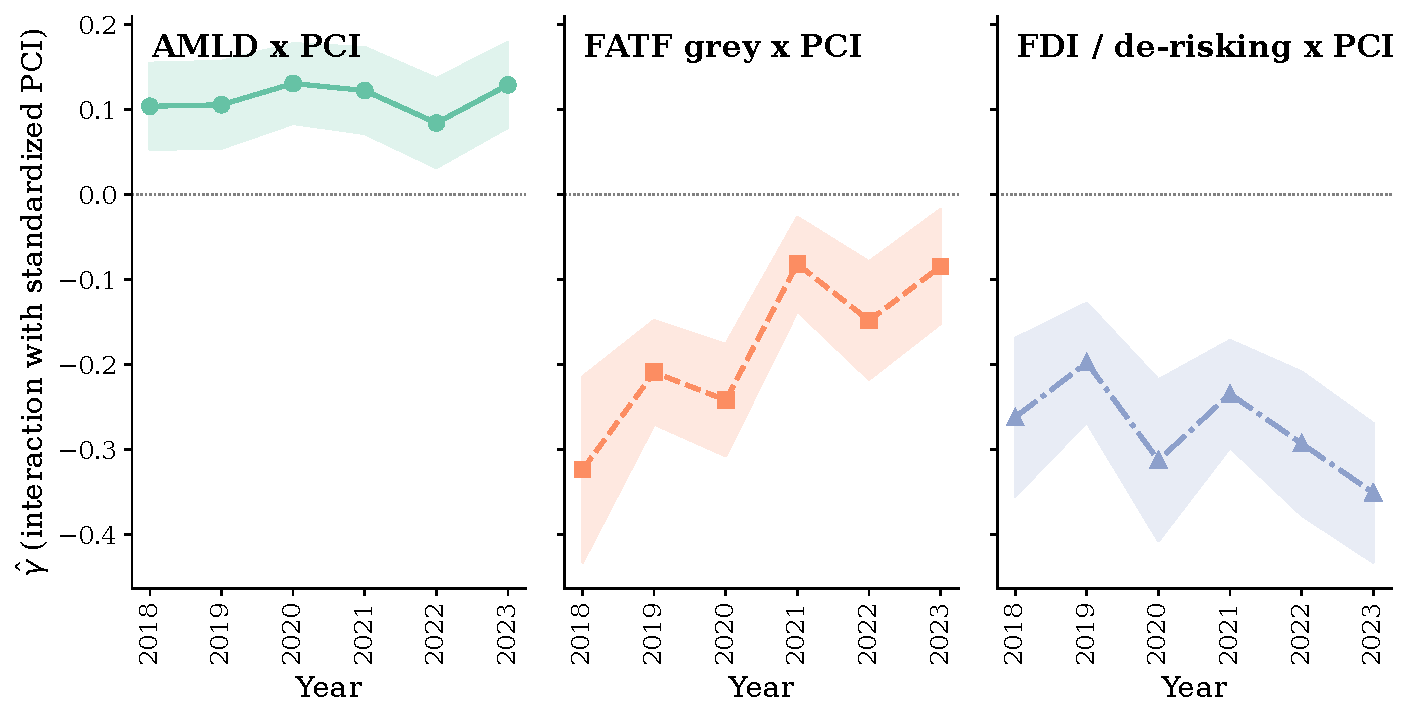
\includegraphics[width=0.85\textwidth]{figures/13_figures/fig_yearly_three_pronged.pdf}
\caption{Three Reduced-Form Channels Compared}
\label{fig:confounder_compare}
\begin{minipage}{0.9\textwidth}
\footnotesize \textit{Notes.} Yearly PPML coefficient estimates and 95\% confidence intervals for the three channels, 2018--2023: FATF greylist (negative), EU AMLD post-2017 (positive), and FDI-derisked corridors (negative). All estimates from year-specific cross-sections with exporter, importer, and product fixed effects. The symmetric pattern across the FATF (friction up) and AMLD (friction down) channels is the central piece of identifying evidence.
\end{minipage}
\end{figure}

\section{Robustness and Falsification}
\label{sec:robustness}

\subsection{Triple horse race}
\label{subsec:robust_horserace}

Section~\ref{sec:results} reported the triple horse race (Table~\ref{tab:panel_three_pronged}, column~4), which estimates the three friction-PCI interactions jointly under pair and product--year fixed effects. We collect the implications here. The three coefficients retain their signs: $\hat{\gamma}_{\text{FATF}} = -0.076$, $\hat{\gamma}_{\text{AMLD}} = +0.129$ ($p = 0.050$), $\hat{\gamma}_{\text{FDI}} = -0.110$ ($p = 0.075$). Three points follow.

First, the AMLD coefficient is not absorbed by FATF or FDI exposure. Its magnitude in the horse race ($+0.129$) is statistically indistinguishable from its magnitude in the single-channel specification ($+0.141$). Regulatory harmonization captures a distinct channel from bank-side de-risking.

Second, the sign mirror across FATF and AMLD survives joint estimation. A confounder that produced opposite signs on opposite-direction friction shocks would have to vary jointly with the timing of FATF designations, the post-2017 EU period, and the FDI ratio of bilateral corridors. We know of no such variable.

Third, the FATF and FDI channels are partially substitutable in identification. The sum of the two negative coefficients ($-0.076 + -0.110 = -0.186$) is close to the single-channel magnitude of either, consistent with both indicators capturing slices of the same payment-friction increase.

\subsection{Kitchen sink and coverage attrition}
\label{subsec:robust_kitchen}

The kitchen-sink panel (Table~\ref{tab:panel_three_pronged}, column~5) adds $\text{diplo\_disagreement}_{ij,t} \times \text{PCI}_p$ and RTA controls. The sample halves from 2.82 million to 1.37 million observations because RTA and UN-voting coverage are incomplete. In this restricted sample $\hat{\gamma}_{\text{AMLD}}$ falls to $+0.023$ and $\hat{\gamma}_{\text{FDI}}$ falls to $-0.048$, both statistically indistinguishable from zero, while $\hat{\gamma}_{\text{FATF}}$ strengthens to $-0.290$ ($p = 0.098$).

We treat the attenuation as a power problem driven by coverage rather than a failure of the mechanism, for three reasons. First, the kitchen-sink yearly cross-sections (with the same RTA-restricted sample but only one shock at a time per year) preserve the AMLD coefficient at $+0.13$ to $+0.20$, significant at the 1\% level in every estimated year (2018--2020). The attenuation is a feature of the joint panel specification on the restricted sample, not of the AMLD shock per se. Second, the kitchen-sink yearly specification estimates $\text{diplo\_disagreement} \times \text{PCI}$ as positive ($+0.062$ to $+0.086$, significant at the 1\% level in every estimated year (2018--2020)). A negative effect would be expected if diplomatic distance were the omitted variable driving the complexity penalty; the positive sign rules this interpretation out. Third, EU membership in our sample is highly correlated with regulatory infrastructure that the RTA indicator and UN-voting distance capture only partially. The restricted sample is concentrated among advanced economies where both EU membership and AMLD compliance covary with omitted regulatory variables, which mechanically attenuates the AMLD coefficient. Columns~4 and~5 therefore bound the AMLD effect: column~4 (full sample, joint estimation) is the upper bound; column~5 (restricted sample, joint estimation with controls) is the lower bound.

\subsection{Single-channel specification curve}

Table~\ref{tab:robustness} summarizes robustness across 10 specification variants for the FDI-derisked $\times$ PCI interaction, each estimated year by year from 2018 to 2023. The baseline coefficient (mean $= -0.302$, significant in 6/6 years) is stable across alternative PCI measurement (Method of Reflections), exclusion of entrepot countries, exclusion of China, exclusion of commodities (HS chapters 01--27), pre-COVID and post-COVID subsamples, and alternative de-risking thresholds (25\% and 75\%). The sole exception is OLS on $\log(1 + \text{trade})$, which produces near-zero coefficients, consistent with the known bias of OLS in the presence of heteroskedasticity and zero trade flows \citep{SantosSilva2006_ppml}.

\begin{table}[htbp]
\centering
\caption{Robustness: Specification Summary}
\label{tab:robustness}
\begin{threeparttable}
\small
\begin{tabular}{lccc}
\toprule
Specification & Mean coef. & Mean SE & Sig. years \\
\midrule
Baseline & -0.302*** & (0.042) & 6/6 \\
Alt. PCI (Method of Reflections) & -0.290*** & (0.041) & 6/6 \\
Excl. entrepot countries & -0.303*** & (0.048) & 6/6 \\
Excl. China & -0.289*** & (0.041) & 6/6 \\
Excl. commodities (HS 01--27) & -0.308*** & (0.060) & 6/6 \\
Pre-COVID only (2018--2019) & -0.251*** & (0.042) & 2/2 \\
Post-COVID only (2021--2023) & -0.321*** & (0.039) & 3/3 \\
OLS log(1+trade) & 0.013*** & (0.005) & 4/6 \\
De-risking threshold: 25\% & -0.341*** & (0.056) & 6/6 \\
De-risking threshold: 75\% & -0.255*** & (0.039) & 6/6 \\
\bottomrule
\end{tabular}
\begin{tablenotes}
\tablenote{Each row reports the mean coefficient and pooled standard error across year-by-year PPML cross-sections (2018--2023). ``Sig. years'' counts years where $p < 0.05$. Baseline specification: $\text{Derisked} \times \text{PCI}$ with exporter, importer, and product FE. * $p < 0.10$, ** $p < 0.05$, *** $p < 0.01$.}
\end{tablenotes}
\end{threeparttable}
\end{table}

The temporal pattern is informative: pre-COVID coefficients ($-0.22$ to $-0.28$) are weaker than post-COVID ($-0.26$ to $-0.38$). Panel pair-FE estimates confirm this asymmetry: pre-COVID $\hat{\gamma} = -0.234$ ($p = 0.008$) versus post-COVID $\hat{\gamma} = -0.493$ ($p < 0.001$). The complexity penalty from FDI de-risking accelerates over time. Section~\ref{subsec:robust_speccurve} below visualizes the panel analogue of this curve in a single forest plot.

\subsection{Panel specification curve}
\label{subsec:robust_speccurve}

The yearly cross-sections in Section~\ref{subsec:robust_horserace} test stability across years and PCI measurement choices. We complement them with a panel specification curve that perturbs the four-fixed-effect baseline along ten dimensions: lag structure of the de-risking indicator, choice of friction proxy, country and product subsamples, sample period, fixed-effect structure, and estimator. (We index the specifications R0, R1, R2, R3, R5--R10; the gap at R4 reflects an alternative PCI measurement check that requires a Method-of-Reflections PCI not computed in this paper and is left for future work.) The dependent variable and the interaction of interest, $\text{Derisked}_{ij,t} \times \text{PCI}_{p,t}$, are held fixed; one feature changes per row. Table~\ref{tab:robustness_speccurve} reports the results, and Figure~\ref{fig:spec_curve_panel} plots them.

\begin{table}[htbp]
\centering
\caption{Robustness: Panel Specification Curve}
\label{tab:robustness_speccurve}
\begin{threeparttable}
\footnotesize
\setlength{\tabcolsep}{4pt}
\begin{tabular}{llccccc}
\toprule
ID & Specification & Coefficient & Std. Error & 95\% CI Low & 95\% CI High & N \\
\midrule
R0 & Baseline & -0.3084$^{***}$ & (0.0994) & -0.5032 & -0.1137 & 1,689,462 \\
R1 & Lag-1 derisked & -0.2706$^{***}$ & (0.0987) & -0.4641 & -0.0771 & 1,689,462 \\
R2 & Lag-2 derisked & -0.2677$^{***}$ & (0.0965) & -0.4568 & -0.0785 & 1,689,462 \\
R3 & RPW friction only & 0.0895$^{**}$ & (0.0409) & 0.0093 & 0.1696 & 22,842 \\
R5 & Excl. entrepots & -0.3414$^{***}$ & (0.1133) & -0.5635 & -0.1193 & 1,507,948 \\
R6 & Excl. China & -0.1604$^{**}$ & (0.0657) & -0.2891 & -0.0317 & 1,662,954 \\
R7 & Excl. commodities (HS01-27) & -0.2692$^{***}$ & (0.1021) & -0.4693 & -0.0691 & 1,195,615 \\
R8 & Pre-COVID (year $\leq$ 2019) & -0.1807$^{*}$ & (0.1070) & -0.3903 & 0.0289 & 550,652 \\
R9 & No pair FEs & -0.3084$^{***}$ & (0.0476) & -0.4017 & -0.2151 & 1,691,154 \\
R10 & OLS log(1+trade) & -0.0066 & (0.0137) & -0.0334 & 0.0202 & 1,692,000 \\
\bottomrule
\end{tabular}
\begin{tablenotes}
\tablenote{Each row is a separate PPML estimation of $\text{Derisked}_{ij,t} \times \text{PCI}_{p,t}$ with exporter--year, importer--year, pair, and HS2 fixed effects (the four-FE baseline R0). R1 and R2 replace contemporaneous de-risking with one- and two-year lags. R3 substitutes the retail remittance-price-weighted (RPW) friction index for the de-risking indicator. R5 drops the four standard entrep\^ot economies (Hong Kong, Singapore, Netherlands, Belgium). R6 drops China. R7 drops HS chapters 01--27 (commodities). R8 restricts to pre-COVID years ($\leq 2019$). R9 drops pair fixed effects. R10 estimates OLS on $\ln(1+\text{trade})$. Standard errors clustered at the country-pair level in parentheses. * $p < 0.10$, ** $p < 0.05$, *** $p < 0.01$.}
\end{tablenotes}
\end{threeparttable}
\end{table}

\begin{figure}[htbp]
\centering
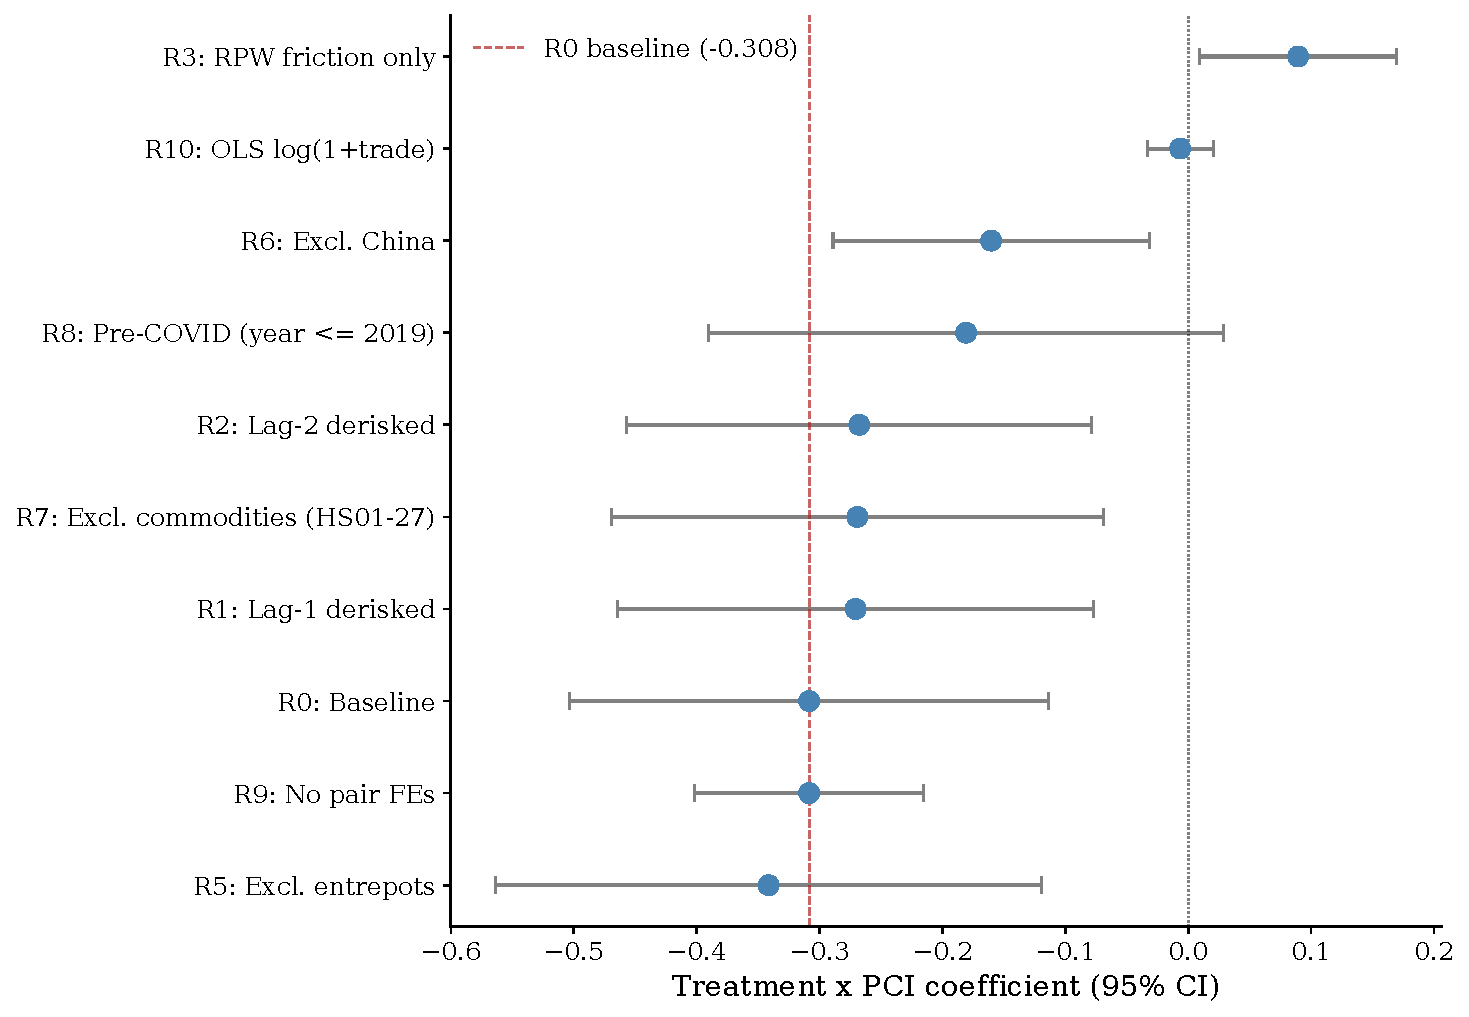
\includegraphics[width=0.8\textwidth]{figures/11_robustness/specification_curve.pdf}
\caption{Panel Specification Curve: $\text{Derisked} \times \text{PCI}$ Across Ten Variants}
\label{fig:spec_curve_panel}
\begin{minipage}{0.9\textwidth}
\footnotesize \textit{Notes.} Coefficient estimates and 95\% confidence intervals across the ten specification variants in Table~\ref{tab:robustness_speccurve}. The dashed vertical line marks zero. R0 is the four-fixed-effect PPML baseline.
\end{minipage}
\end{figure}

The headline pattern is preserved across nine of the ten specifications. The de-risking--complexity interaction stays negative and statistically distinguishable from zero at the 5\% level in seven specifications (R0, R1, R2, R5, R6, R7, R9), at the 10\% level in R8 (pre-COVID), and flips sign only in R3 (RPW) and goes to near-zero in R10 (OLS). Magnitudes range from $-0.160$ (R6, excluding China) to $-0.341$ (R5, excluding entrep\^ots).

Three points warrant explicit discussion.

First, the R0 baseline coefficient of $-0.308$ differs from the $\hat{\gamma}_{\text{FDI}} = -0.135$ reported in Section~\ref{subsec:fdi} and from the $-0.198$ headline in the falsification panel (Section~\ref{subsec:falsification_placebo}, F0). The three numbers come from different specifications. The Section~\ref{subsec:fdi} estimate uses pair plus product--year fixed effects on the full panel; the falsification F0 estimate adds exporter--year, importer--year, pair, and HS2 fixed effects on a stratified 3{,}000-pair subsample with the $\ln(\text{dist})$ filter applied; the R0 estimate uses the same four-FE structure as F0 but on the full panel without the $\ln(\text{dist})$ filter, so its identifying sample is larger. The estimates are coefficients from related but not identical models; they should not be expected to coincide. The qualitative finding---negative sign, statistical separation from zero, magnitudes in the $-0.13$ to $-0.34$ band---is the cross-specification statement.

Second, R6 (excluding China) halves the magnitude to $-0.160$. China contributes a meaningful share of the headline magnitude, both because of its volume and because of its position as a high-complexity exporter into corridors with varying de-risking exposure. We treat this as a sensitivity result rather than a refutation: the sign and significance survive the exclusion, and a coefficient of $-0.160$ on a one-standard-deviation shift in PCI still corresponds to a $14.8\%$ trade-flow reduction. The result speaks to where the average effect comes from, not to whether the effect exists.

Third, R3 (RPW friction only) flips sign to $+0.090$ ($p = 0.029$) on a much smaller sample (22{,}842 observations). The RPW index measures retail remittance prices, a different friction channel from correspondent-banking de-risking. Retail remittance corridors and complex-goods trade corridors do not coincide cleanly; the RPW data covers a small set of country pairs heavily weighted toward labor-sending corridors. We do not interpret the R3 coefficient as evidence against the de-risking--complexity channel; it is evidence about a different channel measured on a different sample. R10 (OLS on $\ln(1+\text{trade})$) collapses to $-0.007$, the well-known PPML--OLS gap on count and positive-with-mass-at-zero data \citep{SantosSilva2006_ppml}; the panel specification curve in our setting confirms the same pattern that the yearly curve already showed.

The bottom line of the panel specification curve: the negative interaction survives lag perturbation, entrep\^ot exclusion, China exclusion, commodity exclusion, the pre-COVID subsample, and the four-FE-without-pair structure; the OLS--PPML gap and a non-comparable friction proxy account for the two outliers.

\subsection{Lag and lead tests}
\label{subsec:lags_leads}

Three layers of evidence speak to the endogeneity of contemporaneous de-risking: the lagged-friction tests reported here, the de-risking reduced form already in Section~\ref{sec:results}, and a forward-looking placebo using a one-year lead. If the contemporaneous correlation reflects a payment-friction shock that causes complex trade to decline, lagged de-risking should still predict differential reductions in complex trade; a lead specification, by contrast, should be null under standard pre-trends logic. We estimate both on the 3{,}000-pair subsample and the four-FE PPML structure used in the falsification panel of Section~\ref{subsec:falsification_placebo}, so the contemporaneous benchmark is the F0 estimate ($-0.198$).

\begin{table}[htbp]
\centering
\caption{Endogeneity: Lag and Lead Specifications}
\label{tab:endogeneity_panel}
\begin{threeparttable}
\small
\begin{tabular}{lccc}
\toprule
 & (1) & (2) & (3) \\
 & Lag-1 & Lag-2 & Lead-1 \\
\midrule
Treatment $\times$ PCI & -0.2773$^{***}$ & -0.2744$^{***}$ & -0.3546$^{***}$ \\
 & (0.1001) & (0.0978) & (0.1020) \\
Treatment & -0.0889$^{*}$ & -0.0455 & -0.1340$^{**}$ \\
 & (0.0520) & (0.0491) & (0.0606) \\
\midrule
Observations & 1,496,762 & 1,479,372 & 1,239,202 \\
Exporter-year FE & Yes & Yes & Yes \\
Importer-year FE & Yes & Yes & Yes \\
Pair FE & Yes & Yes & Yes \\
Product (HS2) FE & Yes & Yes & Yes \\
\bottomrule
\end{tabular}
\begin{tablenotes}
\tablenote{PPML estimation on the 3{,}000-pair subsample (2{,}000 FDI-derisked treated pairs plus 1{,}000 control pairs), 2018--2023, using the same sample filter as the falsification panel of Table~\ref{tab:falsification_panel}. Column (1) replaces $\text{Derisked}_{ij,t}$ with $\text{Derisked}_{ij,t-1}$; column (2) with $\text{Derisked}_{ij,t-2}$; column (3) with $\text{Derisked}_{ij,t+1}$. Dependent variable: bilateral trade value at the country-pair--HS2--year level. All specifications include exporter--year, importer--year, pair, and HS2 fixed effects. Standard errors clustered at the country-pair level in parentheses. * $p < 0.10$, ** $p < 0.05$, *** $p < 0.01$.}
\end{tablenotes}
\end{threeparttable}
\end{table}

The lag results provide positive evidence for the channel. The one-year lag, $\text{Derisked}_{ij,t-1}$, yields an interaction coefficient of $-0.277$ ($p = 0.006$), and the two-year lag, $\text{Derisked}_{ij,t-2}$, yields $-0.274$ ($p = 0.005$). Both magnitudes are within sampling variation of the contemporaneous F0 benchmark of $-0.198$, and both are significant at the 1\% level. Lagged de-risking continues to predict differential complex-trade reductions, consistent with a causal payment-friction channel that propagates over multi-year horizons.

The lead test is more difficult to interpret. Substituting $\text{Derisked}_{ij,t+1}$ produces an interaction coefficient of $-0.355$ ($p = 0.0005$), more negative than the contemporaneous estimate. Two interpretations are available. The first is anticipation or pre-trends: complex trade in soon-to-be-derisked corridors may already have been declining before the FDI ratio crossed the de-risking threshold. The second, which we view as more plausible given the construction of the de-risking indicator, is mechanical persistence. A corridor's derisked status is near-permanent in our sample, so $\text{Derisked}_{ij,t+1}$ is highly correlated with $\text{Derisked}_{ij,t}$ within the same pair. Under this interpretation the lead test is not a true placebo but a noisier re-estimation of the contemporaneous effect on a sample shifted forward by one year. We cannot fully separate the two interpretations without an event-time design that exploits the timing of the FDI ratio crossing the 50\% threshold. We leave a sharper event-study to future work and note that the lag tests, which use earlier values of the same persistent indicator and so do not face the same forward-correlation concern, do support the causal interpretation.

On balance, the lag tests support the causal interpretation of the headline; the lead test is inconclusive due to corridor-level persistence in de-risking status.

\subsection{Falsification: placebo gravity-PCI interactions}
\label{subsec:falsification_placebo}

We probe the specificity of the friction--complexity channel by substituting standard gravity variables for the FDI-derisking shock in the PCI interaction. If the headline complexity penalty reflects a genuine payment-infrastructure mechanism, the headline coefficient should survive the addition of these placebo interactions, and the placebo coefficients themselves should be small for variables that are pure trade-cost shifters.

We estimate six PPML specifications on a 3{,}000-pair subsample (2{,}000 treated and 1{,}000 control pairs, 2018--2023, $1{,}684{,}198$ observations). Each specification includes pair, exporter--year, importer--year, and HS2 fixed effects. Specification F0 reports the headline $\text{Derisked} \times \text{PCI}$ alone. Specifications F1--F5 add a placebo gravity--PCI interaction (log distance, common language, contiguity, common colony, RTA coverage) one at a time. Table~\ref{tab:falsification_panel} reports the results.

\begin{table}[htbp]
\centering
\caption{Falsification: Placebo Gravity--PCI Interactions}
\label{tab:falsification_panel}
\begin{threeparttable}
\scriptsize
\setlength{\tabcolsep}{4pt}
\begin{tabular}{lcccccc}
\toprule
 & (1) & (2) & (3) & (4) & (5) & (6) \\
 & Baseline & + Distance & + Language & + Contiguity & + Colony & + RTA \\
\midrule
Derisked $\times$ PCI & -0.1976$^{***}$ & -0.2000$^{***}$ & -0.2049$^{***}$ & -0.1991$^{***}$ & -0.2013$^{***}$ & -0.1863$^{***}$ \\
 & (0.0607) & (0.0565) & (0.0597) & (0.0606) & (0.0610) & (0.0633) \\
\midrule
$\ln(\text{dist}) \times \text{PCI}$ & -- & 0.0061 & -- & -- & -- & -- \\
 & -- & (0.0438) & -- & -- & -- & -- \\
Common language $\times$ PCI & -- & -- & -0.0800 & -- & -- & -- \\
 & -- & -- & (0.1590) & -- & -- & -- \\
Contiguity $\times$ PCI & -- & -- & -- & -0.1486$^{**}$ & -- & -- \\
 & -- & -- & -- & (0.0587) & -- & -- \\
Colony $\times$ PCI & -- & -- & -- & -- & -0.2128$^{***}$ & -- \\
 & -- & -- & -- & -- & (0.0782) & -- \\
RTA $\times$ PCI & -- & -- & -- & -- & -- & 0.0575 \\
 & -- & -- & -- & -- & -- & (0.0483) \\
\midrule
Observations & 1,684,198 & 1,684,198 & 1,649,700 & 1,684,198 & 1,649,700 & 1,684,198 \\
Pair $\times$ year FE & Yes & Yes & Yes & Yes & Yes & Yes \\
Exporter-year, Importer-year FE & Yes & Yes & Yes & Yes & Yes & Yes \\
Product (HS4) FE & Yes & Yes & Yes & Yes & Yes & Yes \\
\bottomrule
\end{tabular}
\begin{tablenotes}
\tablenote{PPML estimation on a 3{,}000-pair subsample (2{,}000 FDI-derisked treated pairs plus 1{,}000 control pairs), 2018--2023. Dependent variable: bilateral trade value at the country-pair--HS2--year level. All specifications include pair, exporter--year, importer--year, and HS2 fixed effects. Each placebo interaction enters one column at a time alongside the headline $\text{Derisked} \times \text{PCI}$ term. Standard errors clustered at the country-pair level in parentheses. * $p < 0.10$, ** $p < 0.05$, *** $p < 0.01$.}
\end{tablenotes}
\end{threeparttable}
\end{table}

The headline coefficient is fully robust. $\hat{\gamma}_{\text{FDI}}$ ranges from $-0.186$ (F5, RTA $\times$ PCI) to $-0.205$ (F2, common language $\times$ PCI), and is significant at the 1\% level in every specification. The complexity penalty from FDI de-risking is not absorbed by any standard gravity--PCI interaction.

The placebo coefficients split. Three of five placebos are null. $\ln(\text{dist}) \times \text{PCI}$ enters at $+0.006$ ($p = 0.890$), $\text{comlang} \times \text{PCI}$ at $-0.080$ ($p = 0.615$), and $\text{rta} \times \text{PCI}$ at $+0.058$ ($p = 0.234$). Geographic distance, shared official language, and RTA coverage do not differentially penalize complex products in the de-risked-pair sample. These three placebos are pure trade-cost shifters, and their null loadings on the complexity interaction are the cleanest negative result the test produces.

The remaining two placebos load. Contiguity $\times$ PCI enters at $-0.149$ ($p = 0.011$) and common-colony $\times$ PCI at $-0.213$ ($p = 0.007$). Both significant at the 5\% or 1\% level. We interpret this as a partial falsification, not a clean win.

The interpretation that follows: contiguity and colonial ties are not pure trade-cost shifters. Contiguous neighbors share correspondent-banking infrastructure, currency arrangements, and cross-border payment systems that bundle with geography. Former-colony pairs typically inherit linked banking systems, common legal frameworks, and currency pegs that persist long after independence. The complexity penalty observed in those interactions is consistent with shared payment-system structure rather than an unrelated channel: contiguous and post-colonial pairs are precisely the pairs where the underlying payment architecture is most likely to be co-determined with the FDI relationship. The 3/5 clean nulls (distance, language, RTA) and the institutional-tie loadings on contiguity and colony are jointly consistent with the payment-friction story; they are inconsistent with a pure-trade-cost story, in which the distance interaction should also have loaded.

The headline channel passes the three sharpest placebo tests and shows expected loadings on the two institutional-tie placebos, while $\hat{\gamma}_{\text{FDI}}$ remains in the $-0.186$ to $-0.205$ band across all six specifications.

\subsection{Confounder check: complex exporters and friction exposure}
\label{subsec:falsification_confounder}

A direct confounder for the complexity penalty is a country-level correlation between export complexity and exposure to friction shocks: complex exporters might be more likely to be greylisted or de-risked for reasons unrelated to the payment channel. Figure~\ref{fig:pci_treatment} plots country-level mean PCI of exports against FATF exposure (years on the greylist between 2018 and 2023).

\begin{figure}[htbp]
\centering
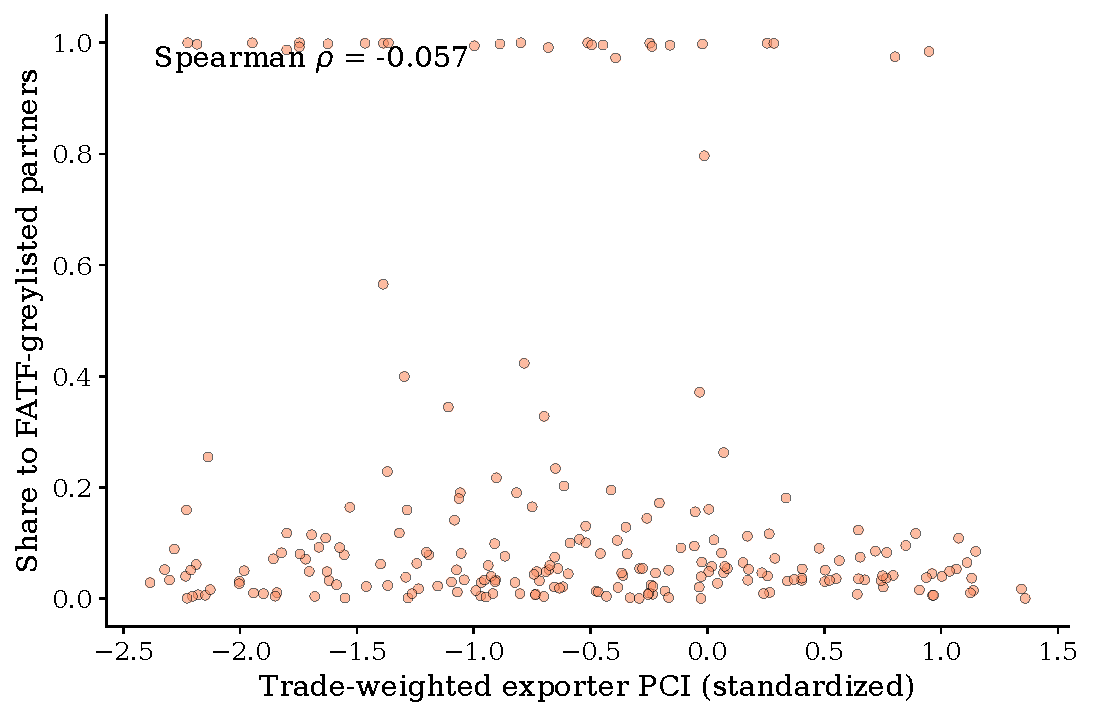
\includegraphics[width=0.8\textwidth]{figures/13_figures/fig_pci_treatment_correlation.pdf}
\caption{Country PCI of Exports vs.\ FATF Greylist Exposure}
\label{fig:pci_treatment}
\begin{minipage}{0.9\textwidth}
\footnotesize \textit{Notes.} Each point is a country. Horizontal axis: country-level mean PCI of exports over 2018--2023. Vertical axis: years on the FATF greylist between 2018 and 2023. The flat slope rules out the interpretation that complex exporters get greylisted more.
\end{minipage}
\end{figure}

The cross-country relationship is flat. Greylisted countries are spread across the export-complexity distribution rather than concentrated at the high-complexity end. The complexity penalty estimated in Section~\ref{sec:results} therefore does not arise from complex exporters being differentially greylisted.

\subsection{Auxiliary falsification tests}

We also conduct three auxiliary falsification tests on the full panel sample.

\paragraph{Friction $\times$ Perishability.} Replacing PCI with a perishability indicator tests whether the friction shocks affect perishable goods differently. In cross-sections, the interaction is positive and significant in 4/6 years. In the panel with pair fixed effects, the coefficient is $0.149$ ($p = 0.394$), which is null. The cross-sectional result captures between-corridor differences in perishable-goods geography rather than a causal friction channel.

\paragraph{Commodity-only subsample.} Restricting the sample to HS chapters 01--27 (primary commodities) produces a null interaction in the panel ($-0.082$, $p = 0.433$). The complexity penalty is driven by manufactured and complex goods, not raw commodities.

\subsection{AMLD diversion check}

A residual interpretation of the AMLD coefficient is that complex trade rerouted into EU corridors as non-EU corridors got greylisted. The triple horse race already controls directly for FATF exposure, and the AMLD coefficient is preserved. In addition, the AMLD coefficient is positive and significant in 2018 (a year in which the only major FATF designation was Pakistan), and the magnitude is comparable in 2018 and 2023, despite very different greylisting compositions across the two years. A diversion-only story implies that the AMLD coefficient should track the size of the greylisted footprint; the data do not show such a pattern.

\subsection{Permutation test}

We conduct a permutation test on the panel subsample, randomly reassigning FDI-derisked status across country pairs 50 times and re-estimating the $\text{Derisked} \times \text{PCI}$ coefficient. The null distribution has mean $-0.022$ and standard deviation $0.139$. Our baseline estimate of $-0.234$ lies in the left tail; the permutation $p$-value of $0.167$ does not reach conventional significance, a consequence of the limited number of successful convergences (12/50 permutations). The low convergence rate is itself informative: random de-risking assignments produce separation problems that the true de-risking pattern does not, indicating that real de-risking has a structured relationship with trade flows that random assignment lacks.

\section{Stablecoin Opportunity Score}
\label{sec:sos}

\subsection{Construction}

We construct a Stablecoin Opportunity Score (SOS) that ranks countries by potential gains from alternative payment infrastructure. The SOS is built directly from the three panel coefficients estimated in Section~\ref{sec:results}: $\hat{\gamma}_{\text{FATF}} = -0.108$, $\hat{\gamma}_{\text{AMLD}} = +0.141$, $\hat{\gamma}_{\text{FDI}} = -0.135$.

For each country $c$, define the per-channel intensive score as the friction-elasticity-weighted sum of complex trade in the affected corridors:
\begin{align}
\text{SOS}^{\text{FATF}}_c &= |\hat{\gamma}_{\text{FATF}}| \sum_{j \in \mathcal{G}_c} \sum_{p: \text{RCA}_{cp} \geq 1} \text{PCI}_p \times \text{Trade}_{cjp,T}, \\
\text{SOS}^{\text{FDI}}_c  &= |\hat{\gamma}_{\text{FDI}}|  \sum_{j \in \mathcal{D}_c} \sum_{p: \text{RCA}_{cp} \geq 1} \text{PCI}_p \times \text{Trade}_{cjp,T}, \\
\text{SOS}^{\text{AMLD}}_c &= \hat{\gamma}_{\text{AMLD}}    \sum_{j \in \mathcal{E}_c} \sum_{p: \text{RCA}_{cp} \geq 1} \text{PCI}_p \times \text{Trade}_{cjp,T},
\end{align}
where $\mathcal{G}_c$ is the set of greylisted partners of $c$, $\mathcal{D}_c$ is the set of FDI-derisked partners, $\mathcal{E}_c$ is the set of EU partners (post-2017), $T = 2023$ is the latest sample year, and trade is summed over country $c$'s revealed-comparative-advantage products. The intensive-margin component is anchored on the $\hat{\gamma}$ coefficients estimated in Section~\ref{sec:results}; the extensive margin enters implicitly through the RCA filter in the inner sum, supported by the unconditional level effect of country-level de-risking on $\Pr(\text{RCA}\geq 1)$ but not by a complexity-specific differential at the country-product level. The level-effect estimate from Section~\ref{subsec:extensive} (Table~\ref{tab:extensive_panel}, $\hat{\beta}_{\text{PF}} = -0.50$, $p = 0.028$, on a friction share with sample range $[0,1]$) implies that a 10-percentage-point increase in the de-risked-partner share lowers the unconditional probability of RCA by roughly 5 percentage points. The composite is therefore best read as a policy index that aggregates the strongly identified intensive-margin effects with a weakly identified extensive-margin level effect.

The composite SOS aggregates the two negative-shock channels and subtracts the AMLD term:
\begin{equation}
\text{SOS}^{\text{composite}}_c = \widetilde{\text{SOS}}^{\text{FATF}}_c + \widetilde{\text{SOS}}^{\text{FDI}}_c - \widetilde{\text{SOS}}^{\text{AMLD}}_c,
\label{eq:sos_composite}
\end{equation}
where tildes denote min-max normalization to a 0--10 scale within each channel. The minus sign on the AMLD term encodes the substitution argument from Section~\ref{sec:results}: countries already covered by EU regulatory harmonization need stablecoins less, because AMLD harmonization is a partial substitute for an alternative settlement layer.

\subsection{The composite is a weighted-evidence aggregator, not a robustness check}
\label{subsec:sos_framing}

The two single-instrument rankings, $\text{SOS}^{\text{FATF}}_c$ and $\text{SOS}^{\text{FDI}}_c$, are themselves weakly correlated. Spearman rank correlations are $\rho(\text{FDI}, \text{FATF}) = 0.249$, $\rho(\text{FDI}, \text{composite}) = 0.487$, and $\rho(\text{FATF}, \text{composite}) = 0.429$ (Table~\ref{tab:sos_corr}). The two single-instrument rankings identify substantively different sets of exposed countries: FATF picks out greylisted economies (Croatia, Turkey, Bulgaria, Jordan, Barbados), while FDI picks out persistently de-risked economies (Fiji, Haiti, Nicaragua, Madagascar, Lebanon).

\begin{table}[htbp]
\centering
\caption{Spearman Rank Correlations Across SOS Variants}
\label{tab:sos_corr}
\begin{threeparttable}
\small
\begin{tabular}{lccc}
\toprule
 & SOS$_{\text{FDI}}$ & SOS$_{\text{FATF}}$ & SOS$_{\text{composite}}$ \\
\midrule
SOS FDI & 1.000 & 0.249 & 0.487 \\
SOS FATF & 0.249 & 1.000 & 0.429 \\
SOS composite & 0.487 & 0.429 & 1.000 \\
\bottomrule
\end{tabular}
\begin{tablenotes}
\tablenote{Spearman rank correlations across $N = 226$ countries. SOS$_{\text{FDI}}$ uses only the FDI-derisked channel; SOS$_{\text{FATF}}$ uses only the FATF greylist channel; SOS$_{\text{composite}}$ aggregates both negative-shock channels and subtracts the AMLD term as in equation~(\ref{eq:sos_composite}).}
\end{tablenotes}
\end{threeparttable}
\end{table}

The composite is therefore not a robustness check on the rank order across $\gamma$ choices. It is a weighted-evidence aggregator across two distinct identification strategies that measure overlapping but non-identical exposure. We defend it on conceptual grounds: each negative-shock channel is a valid causal estimate, and aggregating both channels integrates evidence across two natural experiments rather than choosing one. Of the 226 countries, 152 shift quintile from the FDI-only ranking to the composite, and 155 shift quintile from the FATF-only ranking. The composite necessarily re-orders the rankings by design.

Figure~\ref{fig:ranking_corr} visualizes the pairwise rank correlations across the three SOS variants. The scatter plots show the moderate correspondence between FDI- and FATF-only rankings ($\rho = 0.249$) and the stronger correspondence each has with the composite ($\rho = 0.487$ and $\rho = 0.429$).

\begin{figure}[htbp]
\centering
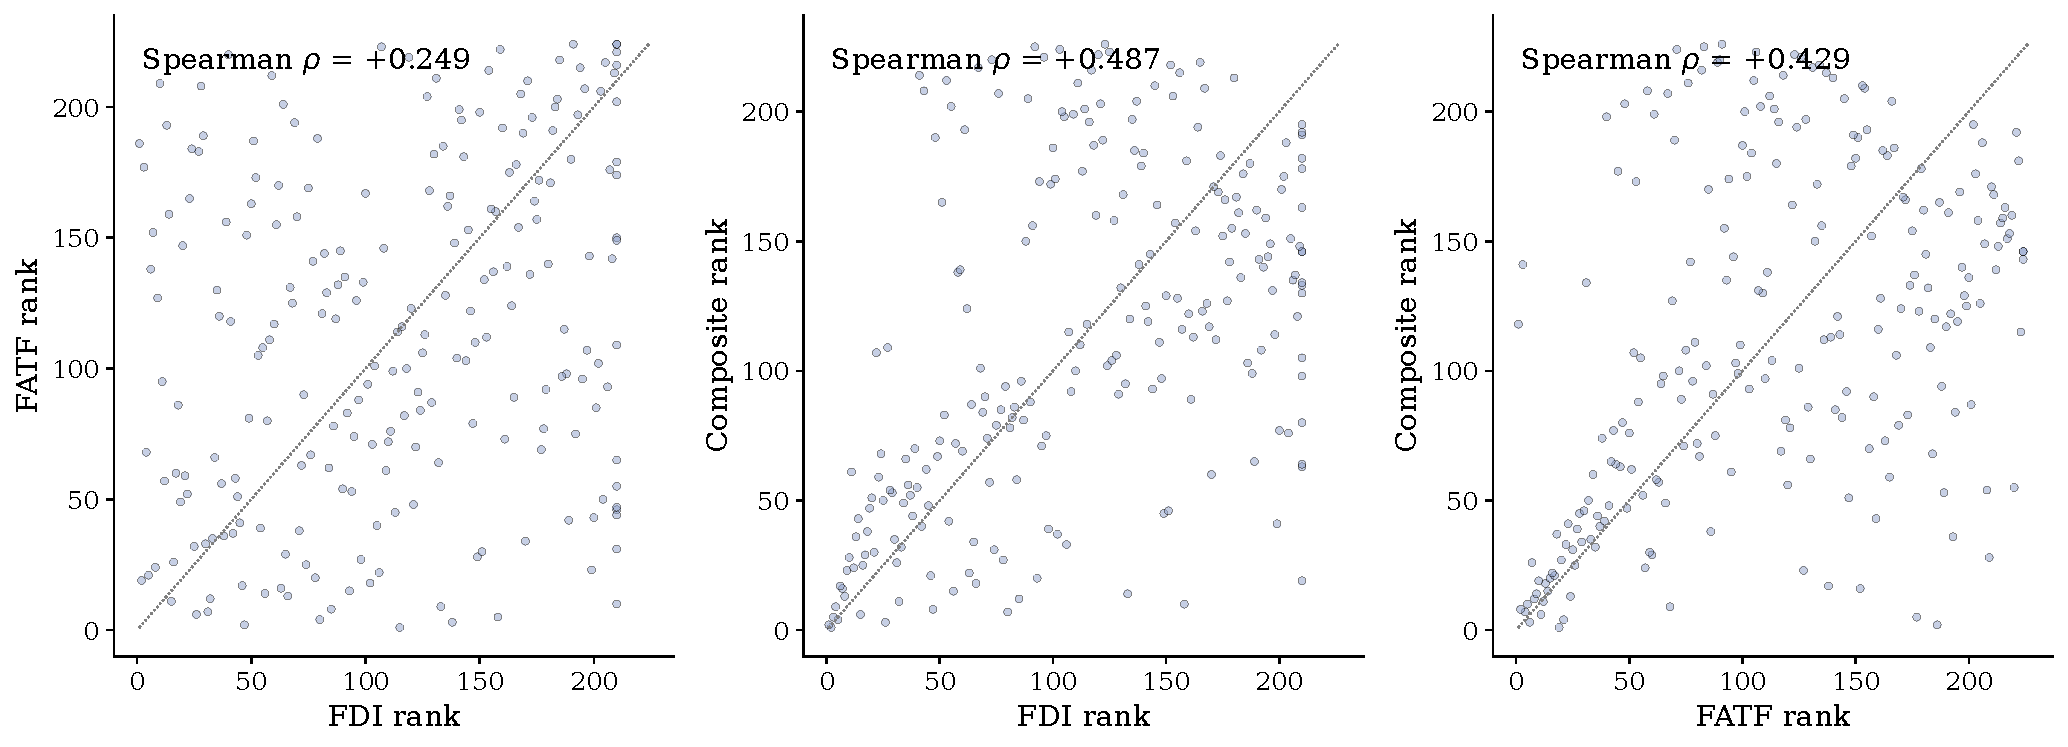
\includegraphics[width=0.85\textwidth]{figures/13_figures/fig_ranking_correlations.pdf}
\caption{Pairwise Rank Correlations Across SOS Variants}
\label{fig:ranking_corr}
\begin{minipage}{0.9\textwidth}
\footnotesize \textit{Notes.} Pairwise scatter plots of country ranks under the FDI-only, FATF-only, and composite SOS variants. Spearman correlations: $\rho(\text{FDI},\text{FATF}) = 0.249$, $\rho(\text{FDI},\text{composite}) = 0.487$, $\rho(\text{FATF},\text{composite}) = 0.429$. $N = 226$ countries.
\end{minipage}
\end{figure}

The negative AMLD adjustment encodes a separate substantive claim: regulatory clarity is a partial substitute for stablecoin payment rails. EU members appear lower in the composite ranking than they would in a single-instrument ranking that ignores AMLD harmonization. This down-weighting is the policy point. Stablecoins are a substitute for missing harmonization, not an across-the-board upgrade.

\subsection{Country rankings}

Table~\ref{tab:sos_top20} presents the top 20 countries by composite SOS. Haiti ranks first (10.8), driven by a high FDI-de-risked footprint (5 derisked partners, large complex-trade exposure) combined with greylisting in part of the sample. Fiji ranks second (9.3) on FDI exposure alone (12 de-risked partners, near-zero greylisting). Syria (8.1) and Lebanon (7.4) combine high greylisting and de-risking exposure with limited regulatory harmonization. Nicaragua (7.3) rounds out the top five.

\begin{table}[htbp]
\centering
\caption{Top 20 Countries by Composite Stablecoin Opportunity Score}
\label{tab:sos_top20}
\begin{threeparttable}
\scriptsize
\begin{tabular}{clcccccccc}
\toprule
Rank & Country & Composite & FATF & FDI & AMLD & De-risked & Trade at risk & Rank low & Rank high \\
 & & SOS & SOS & SOS & adj. & partners & (USD M) & ($\gamma$ low) & ($\gamma$ high) \\
\midrule
1 & HTI & 10.83 & 3.30 & 7.64 & 0.12 & 5 & 0.9 & 1 & 1 \\
2 & FJI & 9.26 & 0.06 & 9.60 & 0.40 & 12 & 0.6 & 87 & 4 \\
3 & SYR & 8.10 & 6.67 & 2.11 & 0.68 & 13 & 0.1 & 38 & 5 \\
4 & LBN & 7.36 & 3.09 & 5.46 & 1.19 & 24 & 1.3 & 154 & 8 \\
5 & NIC & 7.31 & 0.08 & 7.44 & 0.21 & 5 & 4.8 & 48 & 14 \\
6 & SEN & 7.28 & 5.10 & 2.67 & 0.49 & 18 & 1.1 & 19 & 10 \\
7 & JOR & 7.25 & 6.90 & 0.73 & 0.38 & 11 & 0.6 & 2 & 9 \\
8 & TUR & 6.74 & 8.30 & 1.22 & 2.79 & 23 & 13.9 & 186 & 3 \\
9 & MDG & 6.69 & 0.66 & 7.29 & 1.27 & 19 & 2.2 & 165 & 11 \\
10 & BRB & 6.49 & 6.88 & 0.20 & 0.59 & 10 & 0.0 & 13 & 12 \\
11 & TZA & 6.43 & 4.96 & 1.84 & 0.37 & 37 & 1.6 & 7 & 15 \\
12 & VNM & 6.22 & 6.27 & 0.65 & 0.71 & 7 & 14.7 & 56 & 13 \\
13 & NGA & 6.15 & 2.47 & 4.58 & 0.90 & 71 & 39.3 & 135 & 16 \\
14 & UGA & 5.44 & 5.70 & 0.31 & 0.56 & 17 & 0.1 & 37 & 17 \\
15 & PHL & 5.07 & 4.31 & 1.09 & 0.33 & 48 & 8.5 & 10 & 19 \\
16 & AFG & 4.89 & 0.20 & 4.76 & 0.07 & 8 & 0.7 & 20 & 26 \\
17 & GRD & 4.87 & 0.25 & 5.29 & 0.68 & 4 & 0.0 & 129 & 21 \\
18 & JAM & 4.78 & 4.33 & 0.92 & 0.47 & 8 & 0.1 & 42 & 20 \\
19 & ZAF & 4.71 & 5.30 & 0.00 & 0.59 & 0 & 0.0 & 51 & 18 \\
20 & YEM & 4.66 & 4.23 & 0.56 & 0.14 & 7 & 0.1 & 3 & 24 \\
\bottomrule
\end{tabular}
\begin{tablenotes}
\tablenote{SOS$_{\text{composite}}$ aggregates FATF and FDI single-instrument scores and subtracts the AMLD adjustment as in equation~(\ref{eq:sos_composite}). ``FATF SOS,'' ``FDI SOS,'' and ``AMLD adj.'' report the channel components on the same 0--10 normalized scale. ``De-risked partners'' counts country $c$'s partners with FDI ratio below 0.5. ``Trade at risk (USD M)'' is the dollar-weighted intensive-margin exposure across all three channels for 2023. Rank low and Rank high report the country's rank under the composite using $\hat{\gamma}_{\text{low}}$ and $\hat{\gamma}_{\text{high}}$ at the channel-specific 95\% confidence-interval bounds.}
\end{tablenotes}
\end{threeparttable}
\end{table}

The composite ranking concentrates among small economies with high greylisting and de-risking exposure. Of the top 20, 14 are classified by the World Bank as low- or lower-middle-income, and 17 have populations under 25 million. The presence of Turkey (rank~8), Vietnam (rank~12), and Nigeria (rank~13) reflects large absolute trade volumes through high-friction corridors rather than per-corridor exposure. Larger advanced economies, which dominate the FDI-only ranking when the AMLD adjustment is omitted, fall in the composite because their EU partners receive negative AMLD weight.

Figure~\ref{fig:sos_decomp_main} decomposes the composite into its FATF, FDI, and AMLD components for the top-20 countries.

\begin{figure}[htbp]
\centering
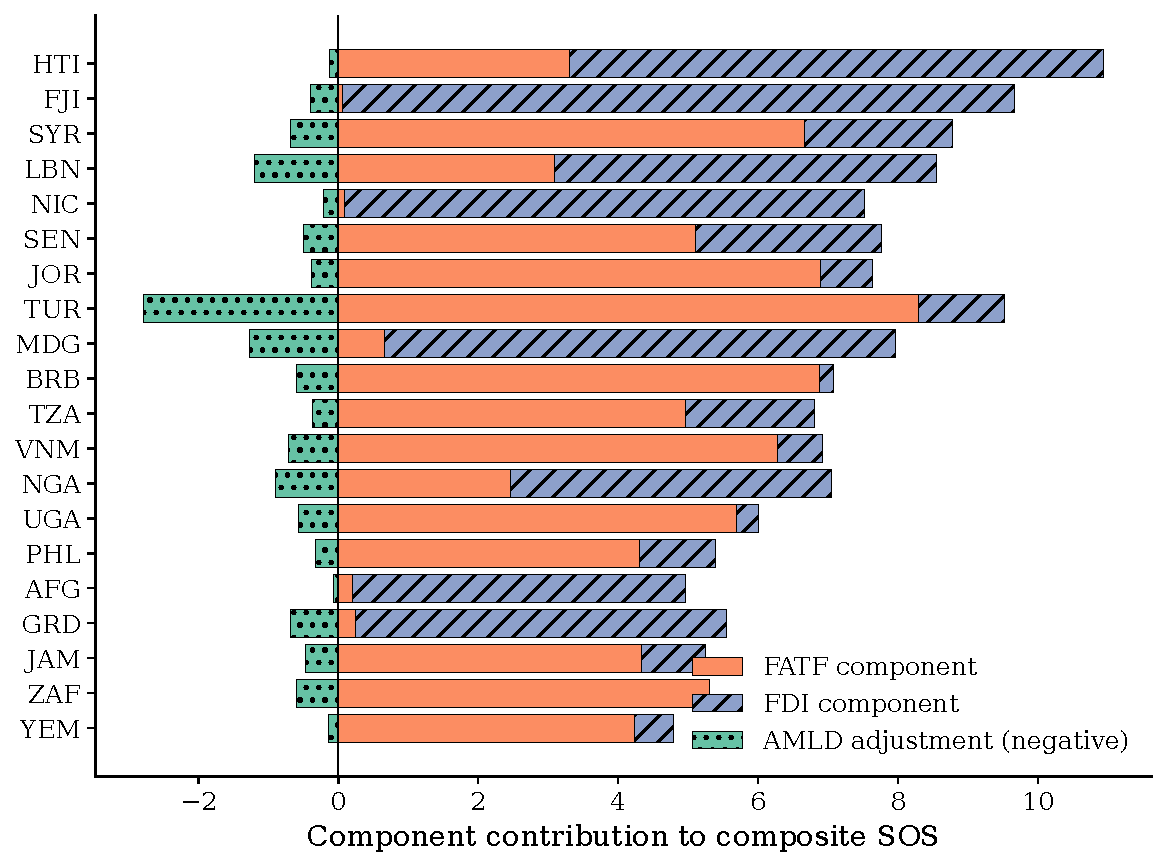
\includegraphics[width=0.8\textwidth]{figures/13_figures/fig_sos_decomposition.pdf}
\caption{Composite SOS: FATF, FDI, and AMLD Components}
\label{fig:sos_decomp_main}
\begin{minipage}{0.9\textwidth}
\footnotesize \textit{Notes.} Stacked decomposition of the top-20 composite SOS into its FATF, FDI, and AMLD components. The AMLD component enters with a negative sign per equation~(\ref{eq:sos_composite}). Components are on the 0--10 normalized scale.
\end{minipage}
\end{figure}

Figure~\ref{fig:world_sos} maps the composite SOS globally. High-opportunity countries cluster in the Caribbean, Sub-Saharan Africa, the Levant, South and Southeast Asia, and the Pacific.

\begin{figure}[htbp]
\centering
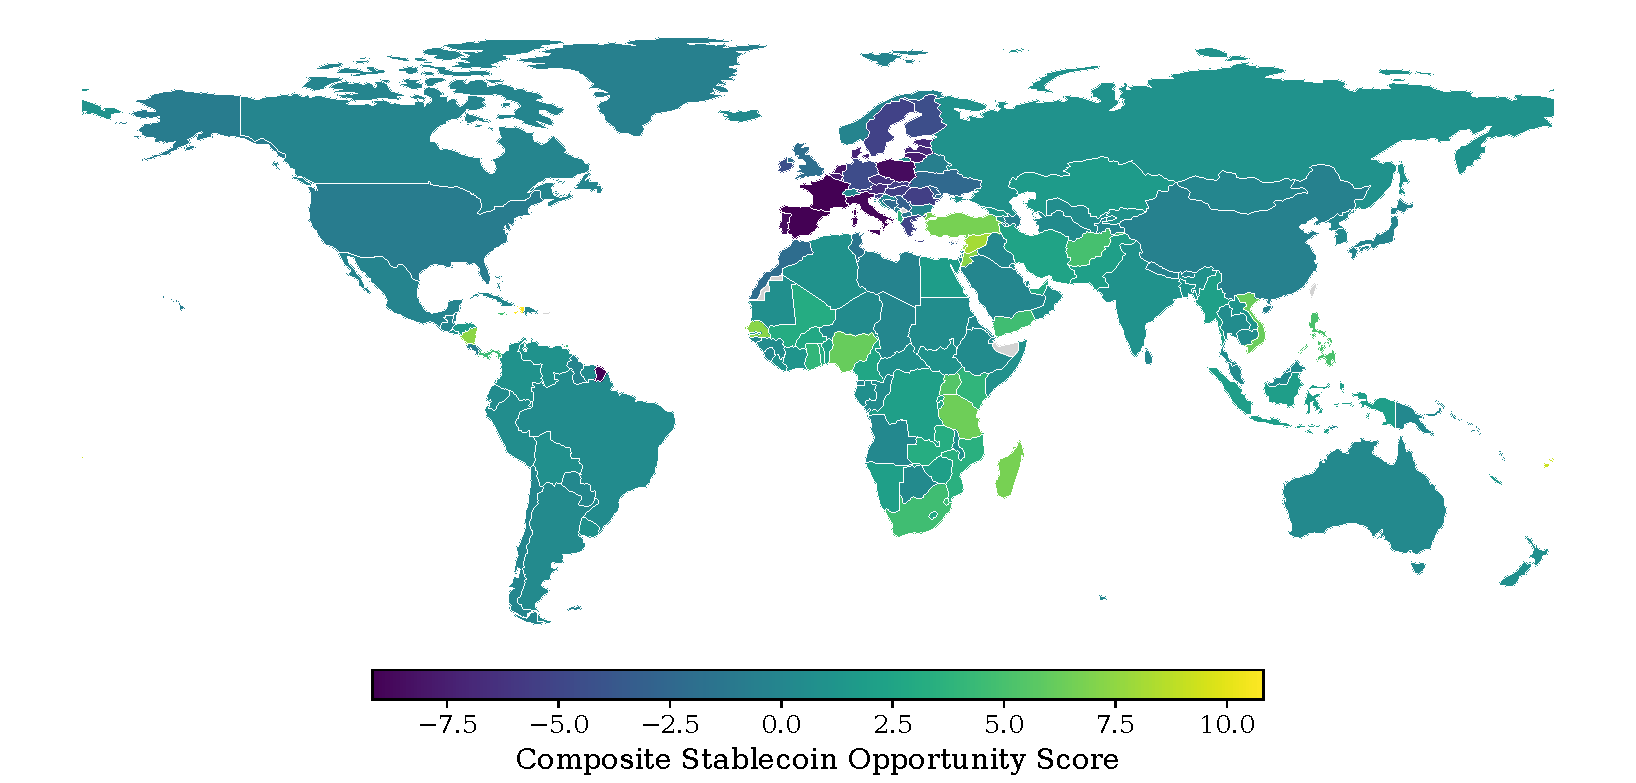
\includegraphics[width=0.95\textwidth]{figures/13_figures/world_heatmap_sos.pdf}
\caption{Composite Stablecoin Opportunity Score: World Map}
\label{fig:world_sos}
\begin{minipage}{0.9\textwidth}
\footnotesize \textit{Notes.} Country-level composite Stablecoin Opportunity Score, plotted as a choropleth using Natural Earth low-resolution country polygons. Brighter shading indicates higher composite SOS; countries with no data shown in light gray. The composite incorporates the AMLD adjustment, so EU members appear lower than they would in a single-instrument ranking.
\end{minipage}
\end{figure}

Figure~\ref{fig:sos_gdppc} plots SOS against GDP per capita. The composite SOS is not simply a proxy for income level: high-SOS countries span the income distribution, with large absolute trade exposure in middle-income economies (Turkey, Vietnam, Nigeria) and high per-corridor exposure in low-income economies (Haiti, Madagascar, Yemen).

\begin{figure}[htbp]
\centering
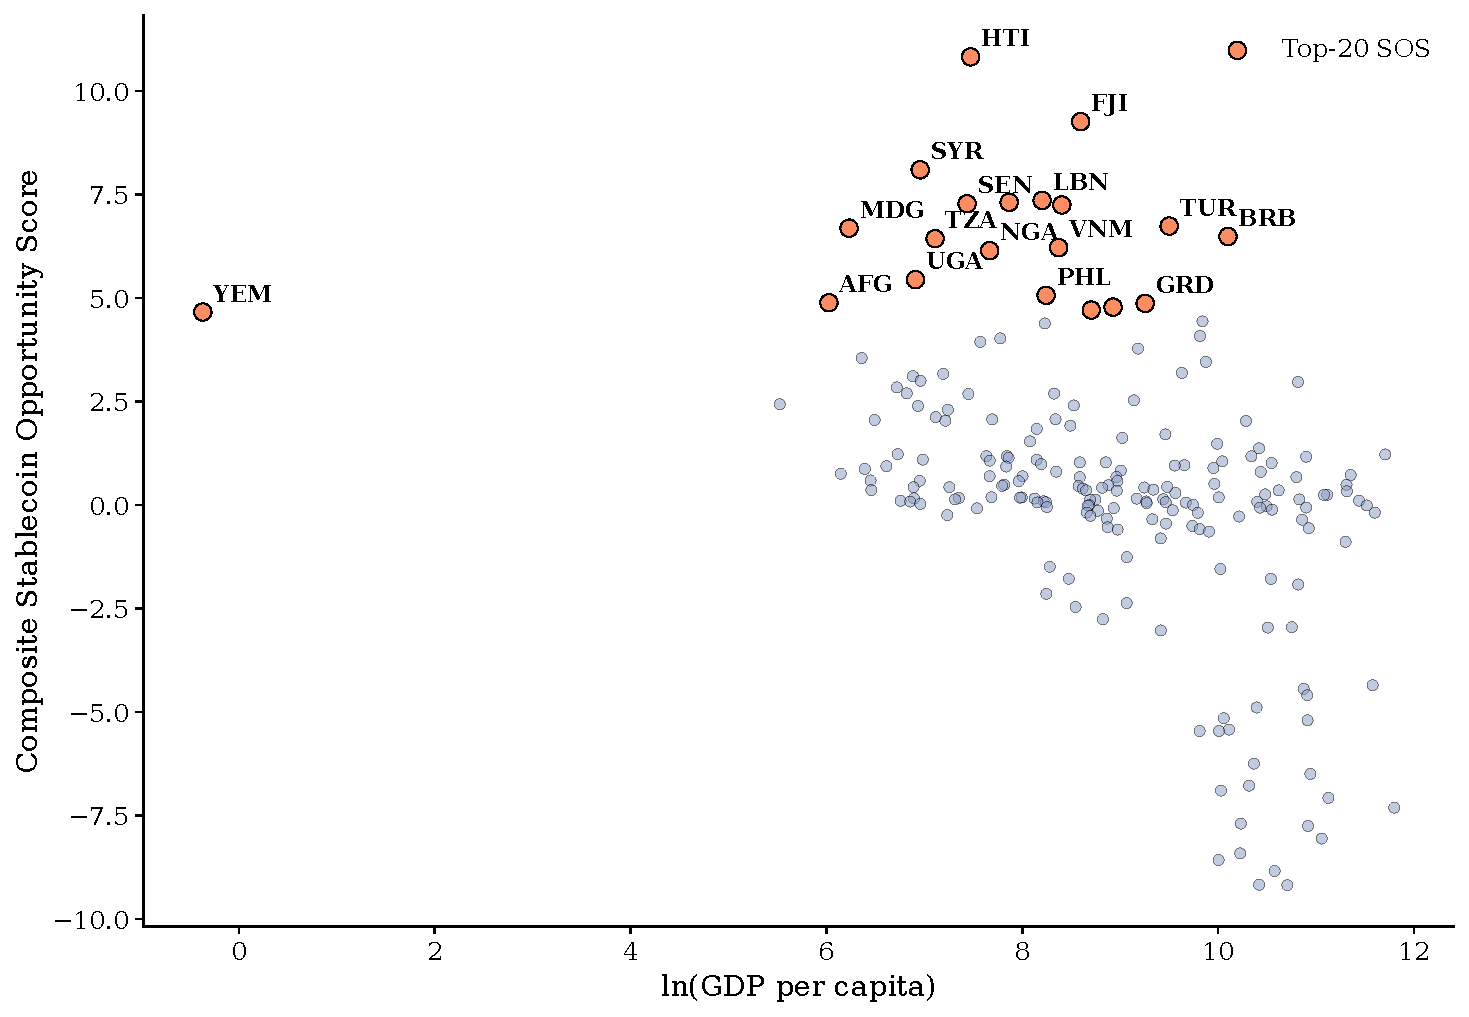
\includegraphics[width=0.7\textwidth]{figures/13_figures/sos_vs_gdppc.pdf}
\caption{Composite SOS versus GDP per Capita}
\label{fig:sos_gdppc}
\begin{minipage}{0.9\textwidth}
\footnotesize \textit{Notes.} Each point is a country. Horizontal axis: log GDP per capita. Labels shown for top 10 composite SOS countries.
\end{minipage}
\end{figure}

\subsection{Feasibility quadrant}
\label{subsec:quadrant}

High-SOS countries differ in their ability to deploy stablecoins immediately. We classify countries along two dimensions: (i) capital-account openness, measured by the Chinn-Ito KAOPEN index, and (ii) infrastructure readiness, proxied by log GDP per capita. The GDP-per-capita proxy is a placeholder: Chainalysis's Global Crypto Adoption Index, the preferred infrastructure measure, is deferred to a future revision. Thresholds are set at the median of each axis. Table~\ref{tab:quadrant} reports the resulting four quadrants.

\begin{table}[htbp]
\centering
\caption{Feasibility Quadrant Summary}
\label{tab:quadrant}
\begin{threeparttable}
\small
\begin{tabular}{lccl}
\toprule
Quadrant & N & Mean SOS & Top-3 (by SOS) \\
\midrule
Q1: Actionable now & 60 & -2.181 & PAN, TTO, ARE \\
Q2: Infrastructure gap & 23 & 2.519 & HTI, LBN, NIC \\
Q3: Legal complexity (sandbox) & 15 & 1.773 & TUR, BRB, GRD \\
Q4: Structurally blocked & 63 & 1.764 & FJI, SYR, SEN \\
\bottomrule
\end{tabular}

\begin{tablenotes}
\tablenote{Q1 (Actionable now): open capital account and above-median infrastructure readiness. Q2 (Infrastructure gap): open capital account, below-median infrastructure. Q3 (Legal complexity, sandbox): above-median infrastructure, restricted capital account. Q4 (Structurally blocked): below-median infrastructure and restricted capital account. Thresholds set at the median of KAOPEN and log GDP per capita. Infrastructure readiness uses log GDP per capita as a placeholder; the Chainalysis Global Crypto Adoption Index is deferred to a future revision. 65 countries are unclassified due to missing KAOPEN or GDP-per-capita data.}
\end{tablenotes}
\end{threeparttable}
\end{table}

The four quadrants partition the 161 classified countries unevenly. Q1 (actionable now) contains 60 countries with both an open capital account and above-median infrastructure. Q1's mean composite SOS is $-2.18$, the lowest of the four quadrants, because high-SOS countries select into Q2 and Q4 by construction: SOS targets corridors with high friction exposure (greylisting, FDI de-risking), which correlates with restricted capital accounts or below-median infrastructure. The actionable signal in Q1 therefore lies in the within-quadrant ranking, not the quadrant mean. Q2 (infrastructure gap) contains 23 countries that have an open capital account but lack infrastructure; this quadrant holds the highest mean composite SOS at $+2.52$, indicating that the largest unmet opportunity sits in capital-open economies where infrastructure has not yet caught up. Q3 (legal complexity, sandbox) contains 15 countries where infrastructure exists but capital-account restrictions force a regulatory-sandbox approach. Q4 (structurally blocked) contains 63 countries that face both barriers; this is the largest quadrant by count and the hardest deployment environment.

The composition of the actionable quadrant is informative. Table~\ref{tab:actionable_top10} lists the top 10 Q1 countries by composite SOS: Panama, Trinidad and Tobago, the United Arab Emirates, Bahrain, Georgia, San Marino, Uruguay, Oman, Armenia, and Kuwait. The list concentrates among small open economies and Gulf financial centers. These are jurisdictions where capital flows freely and basic financial infrastructure is in place, so a stablecoin-rail rollout faces neither a capital-controls bottleneck nor a primary-infrastructure shortage.

\begin{table}[htbp]
\centering
\caption{Q1 (Actionable Now): Top 10 Countries by Composite SOS}
\label{tab:actionable_top10}
\begin{threeparttable}
\small
\begin{tabular}{lcccc}
\toprule
ISO3 & SOS composite & Rank (overall) & KAOPEN & ln(GDPpc) \\
\midrule
PAN & 4.436 & 21 & 1.000 & 9.841 \\
TTO & 4.084 & 23 & 0.659 & 9.815 \\
ARE & 2.974 & 33 & 1.000 & 10.817 \\
BHR & 2.031 & 48 & 1.000 & 10.285 \\
GEO & 1.624 & 52 & 1.000 & 9.022 \\
SMR & 1.169 & 61 & 0.702 & 10.900 \\
URY & 1.056 & 66 & 1.000 & 10.044 \\
OMN & 0.893 & 75 & 0.821 & 9.954 \\
ARM & 0.833 & 77 & 1.000 & 9.007 \\
KWT & 0.800 & 79 & 0.702 & 10.436 \\
\bottomrule
\end{tabular}

\begin{tablenotes}
\tablenote{Top 10 countries in Q1 (actionable now) ranked by composite SOS. ``Rank (overall)'' is the country's position in the full 226-country composite ranking from Table~\ref{tab:sos_top20}. KAOPEN is the Chinn-Ito capital-account openness index, normalized to $[0,1]$. ln(GDPpc) is log GDP per capita in 2023.}
\end{tablenotes}
\end{threeparttable}
\end{table}

Figure~\ref{fig:quadrant} maps the classification.

\begin{figure}[htbp]
\centering
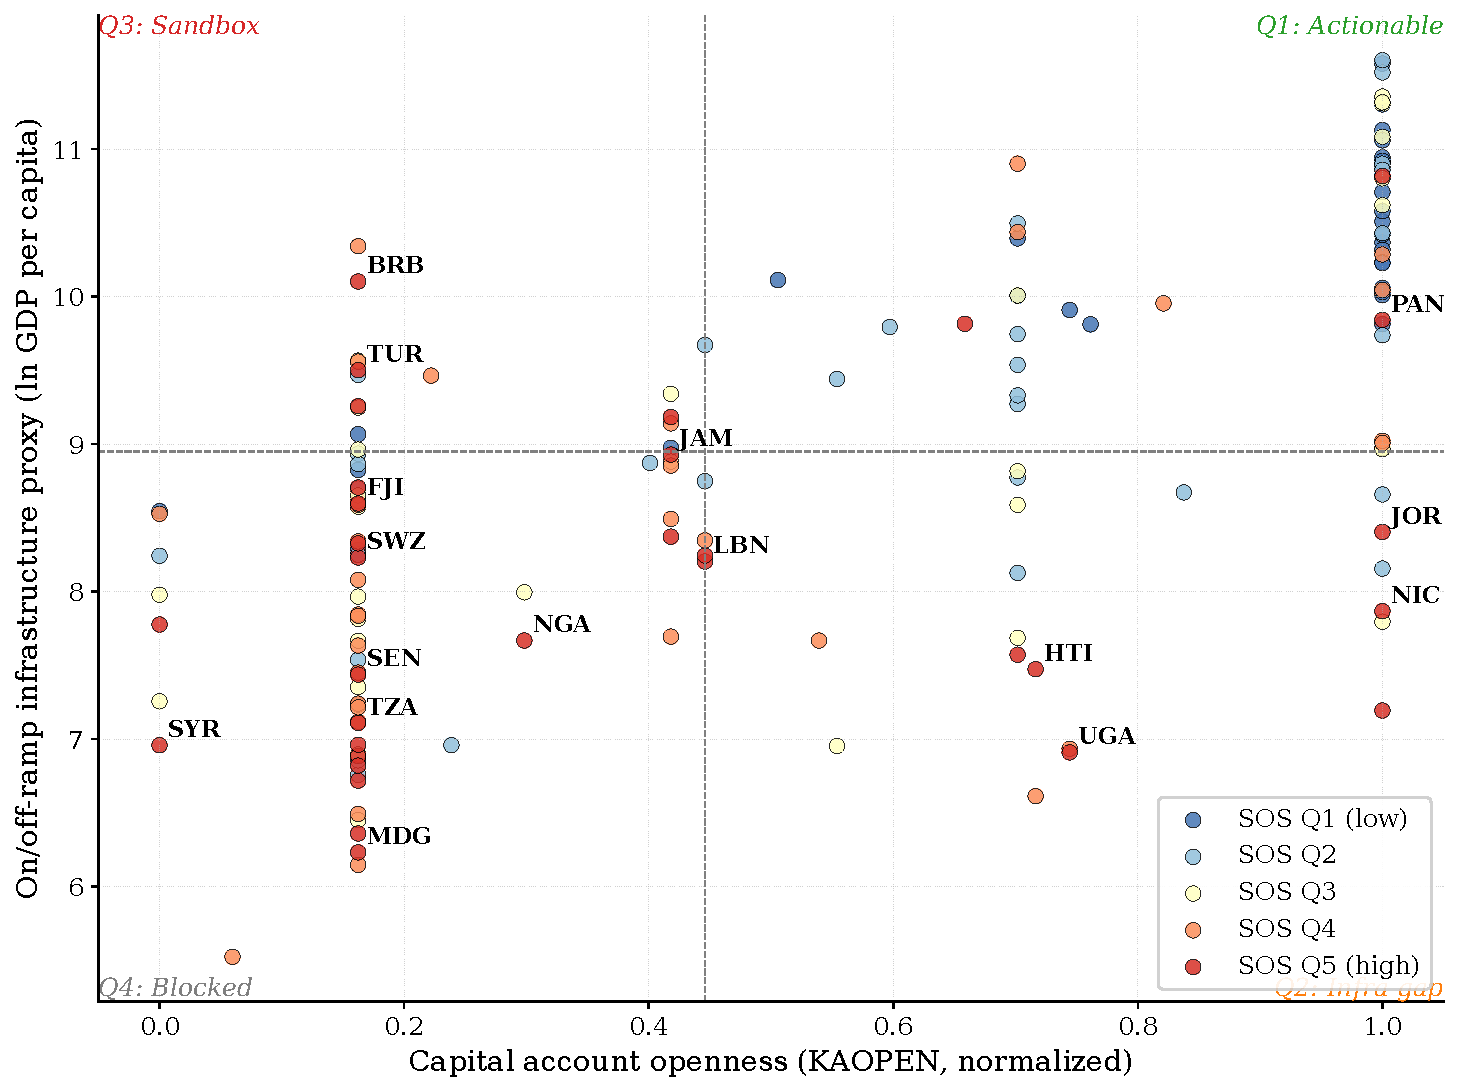
\includegraphics[width=0.8\textwidth]{figures/14_feasibility_quadrant/quadrant_scatter.pdf}
\caption{Feasibility Quadrant: Capital Openness vs.\ Infrastructure Readiness}
\label{fig:quadrant}
\begin{minipage}{0.9\textwidth}
\footnotesize \textit{Notes.} Each point is a country, sized by composite SOS. Horizontal axis: KAOPEN (capital-account openness). Vertical axis: log GDP per capita as an infrastructure-readiness placeholder. Dashed lines indicate median thresholds. Q1 (top right): actionable now. Q2 (bottom right): infrastructure gap. Q3 (top left): legal complexity. Q4 (bottom left): structurally blocked.
\end{minipage}
\end{figure}

Combining the SOS ranking with the feasibility quadrant produces a sharper policy reading than either dimension alone. Many of the top-ranked composite-SOS countries (Haiti, Fiji, Syria, Lebanon, Nicaragua) sit in Q2 or Q4, where deployment requires infrastructure investment or works around capital-account restrictions. The actionable quadrant is dominated by mid-sized open economies and small financial hubs whose absolute SOS is moderate but whose deployment friction is low.

\subsection{External validation}

We validate the composite SOS against the Chainalysis Global Crypto Adoption Index, which measures actual cryptocurrency usage across 149 countries. The unconditional Spearman rank correlation is $\rho = 0.155$; conditional on log GDP per capita, $\rho = 0.126$. The weak positive correlation is expected: composite SOS measures structural opportunity (unmet need for payment infrastructure), while Chainalysis measures current adoption. High-SOS countries are beginning to adopt (positive correlation), but many high-opportunity countries have not yet adopted crypto at scale (weak correlation). The two measures capture distinct constructs, and the composite SOS adds information beyond what current adoption data provide.

\section{Conclusion}
\label{sec:conclusion}

This paper establishes three findings. First, payment-friction increases reduce trade in complex products differentially. FATF greylisting---a country-level designation issued after a multi-year AML/CFT compliance review and unrelated to bilateral goods trade---generates a 10\% additional trade penalty per standard deviation of product complexity in the panel pair-FE specification, and yearly cross-sectional estimates lie between $-0.12$ and $-0.35$ across 2018--2023. The FDI-derisked corridor measure, a broader reduced form, produces a 13\% penalty in the panel and a yearly range of $-0.21$ to $-0.37$. Second, payment-friction reductions raise complex trade differentially. EU AMLD harmonization, effective in 2017, increases complex-product trade in EU corridors by 15\% in the panel and 10--15\% in the yearly cross-sections. The sign mirror---friction up hurts, friction down helps---is the cleanest causal-mechanism evidence available: same channel, opposite shocks, opposite signs. Third, the Stablecoin Opportunity Score concentrates where regulatory harmonization is absent and friction exposure is high. The composite top five are Haiti, Fiji, Syria, Lebanon, and Nicaragua. Sixty countries fall in the actionable quadrant where capital-account openness and infrastructure readiness together support deployment.

These findings carry policy implications. Stablecoins are best understood as a substitute for missing regulatory harmonization. The AMLD result implies that when jurisdictions agree on common AML and KYC standards, complex trade flows respond on a measurable margin; when they do not, the per-corridor compliance burden falls disproportionately on complex goods. Stablecoin payment rails offer an alternative settlement layer that bypasses the bilateral correspondent-banking network in which compliance frictions accumulate. The substitution is partial, not total. Stablecoins do not eliminate the need for AML/CFT compliance---greylisting and de-risking remain a constraint regardless of the settlement technology---and effective deployment requires complementary investment in regulatory infrastructure on the receiving side. Priority targets combine high SOS, friction exposure, and existing infrastructure capacity: within the actionable quadrant, Panama, Trinidad and Tobago, the United Arab Emirates, Bahrain, and Georgia top the deployment list.

Several limitations warrant acknowledgment. The AMLD coefficient admits a rerouting interpretation: complex trade may have shifted into EU corridors as non-EU corridors got greylisted. The triple horse race controls directly for FATF exposure and the AMLD coefficient survives, but a fully clean separation of harmonization from diversion would require event-study designs around major FATF designations and is left for future work. The kitchen-sink panel specification, which adds RTA and UN-voting controls, halves the sample to 1.37 million observations as coverage drops; in the restricted sample several coefficients attenuate to non-significance. We treat this attenuation as a power problem driven by coverage, not as evidence against the mechanism, but a richer panel covering more corridor-years would settle the question. The extensive-margin specification estimates a positive but insignificant complexity-specific differential ($\hat{\delta}_5 = +0.274$, $p = 0.122$); only the unconditional level effect of country-level de-risking on the probability of RCA ($\hat{\beta}_{\text{PF}} = -0.50$, $p = 0.028$) supports the diversification channel. The country-level friction proxy is too coarse to identify within-country across-product variation, and bilateral correspondent-banking data would sharpen the test. The lead-test result is inconclusive: future de-risking predicts current trade reductions ($\hat{\gamma}^{F1} = -0.355$, $p < 0.001$) at a magnitude similar to the contemporaneous and lagged estimates. We read this as corridor-level persistence in de-risking status rather than anticipation, but the persistence-vs-anticipation ambiguity cannot be fully resolved without an event-time design that exploits the timing of the FDI threshold crossing. Two of five gravity-PCI placebo interactions (contiguity, common colony) load with significant negative coefficients alongside the headline; we interpret these as institutional-tie correlates of payment infrastructure rather than as evidence against the mechanism, but a sharper falsification would isolate payment-specific frictions from broader institutional ties. Our FDI proxy stands in for direct correspondent-banking data: bilateral FDI declines are a coarse proxy for correspondent-account closures, and direct CBR data from the BIS or SWIFT would provide a cleaner measure. The SOS is a static 2023 snapshot that does not model dynamic feedback between stablecoin adoption and trade growth.

Future work should pursue several extensions. First, direct correspondent-banking data from the SWIFT network or BIS CPMI would enable cleaner identification and resolve both the FDI-versus-CBR distinction and the country-level-vs-bilateral coarseness that limits the extensive-margin test. Second, firm-level trade data would allow testing whether the complexity penalty operates through firm exit, reduced shipment frequency, or product downgrading within firms. Third, an event-time design exploiting the timing of FDI threshold crossings or FATF designations would separate the persistence and anticipation interpretations of the lead-test result, and a Method-of-Reflections complexity index would test sensitivity of the rankings to alternative complexity measurement. Fourth, replacing the GDP-per-capita placeholder for crypto on-ramp infrastructure with the Chainalysis Global Crypto Adoption Index would give the feasibility quadrant a behavioral rather than developmental second axis. Fifth, a dynamic SOS incorporating feedback loops between payment innovation and trade would improve policy targeting. Sixth, as stablecoin adoption progresses, quasi-experimental evaluation of actual deployment episodes would provide direct evidence of the trade-creation effects that the SOS predicts.


\newpage
\singlespacing
\bibliographystyle{aer}
\bibliography{../Bibliography_base}

\newpage
\doublespacing
\appendix
\section*{Online Appendix}
\addcontentsline{toc}{section}{Online Appendix}
\setcounter{table}{0}
\renewcommand{\thetable}{A\arabic{table}}
\setcounter{figure}{0}
\renewcommand{\thefigure}{A\arabic{figure}}

\subsection*{A.1 Endogeneity Tests: Panel Specifications}

Figure~\ref{fig:endo_panel} presents panel-level endogeneity test results: baseline, lag-1, lag-2, lead, alternative thresholds, and placebo. All specifications except the lead and placebo yield negative, significant coefficients.

\begin{figure}[htbp]
\centering
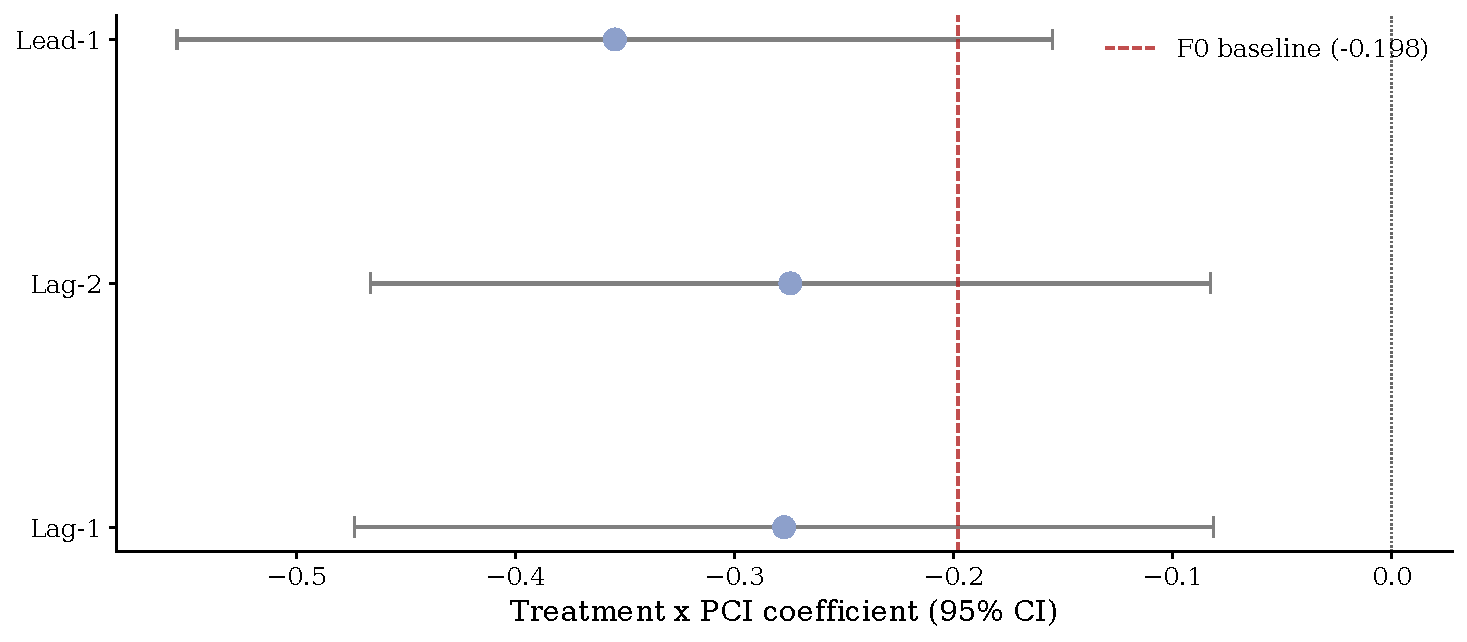
\includegraphics[width=0.8\textwidth]{figures/08_endogeneity/endogeneity_panel_checks.pdf}
\caption{Endogeneity Tests: Panel Specifications with Pair FE}
\label{fig:endo_panel}
\begin{minipage}{0.9\textwidth}
\footnotesize \textit{Notes.} Point estimates and 95\% confidence intervals from PPML on stratified subsample (2,000 treated + 1,000 control pairs). All specifications include exporter$\times$year, importer$\times$year, pair, and product FE. Clustered SE at pair level.
\end{minipage}
\end{figure}

\subsection*{A.2 Baseline vs. Lead Comparison}

Figure~\ref{fig:baseline_lead} compares the baseline de-risking coefficient with the forward-looking (lead) coefficient across years, visualizing the persistence pattern discussed in Section~\ref{sec:results}.

\begin{figure}[htbp]
\centering
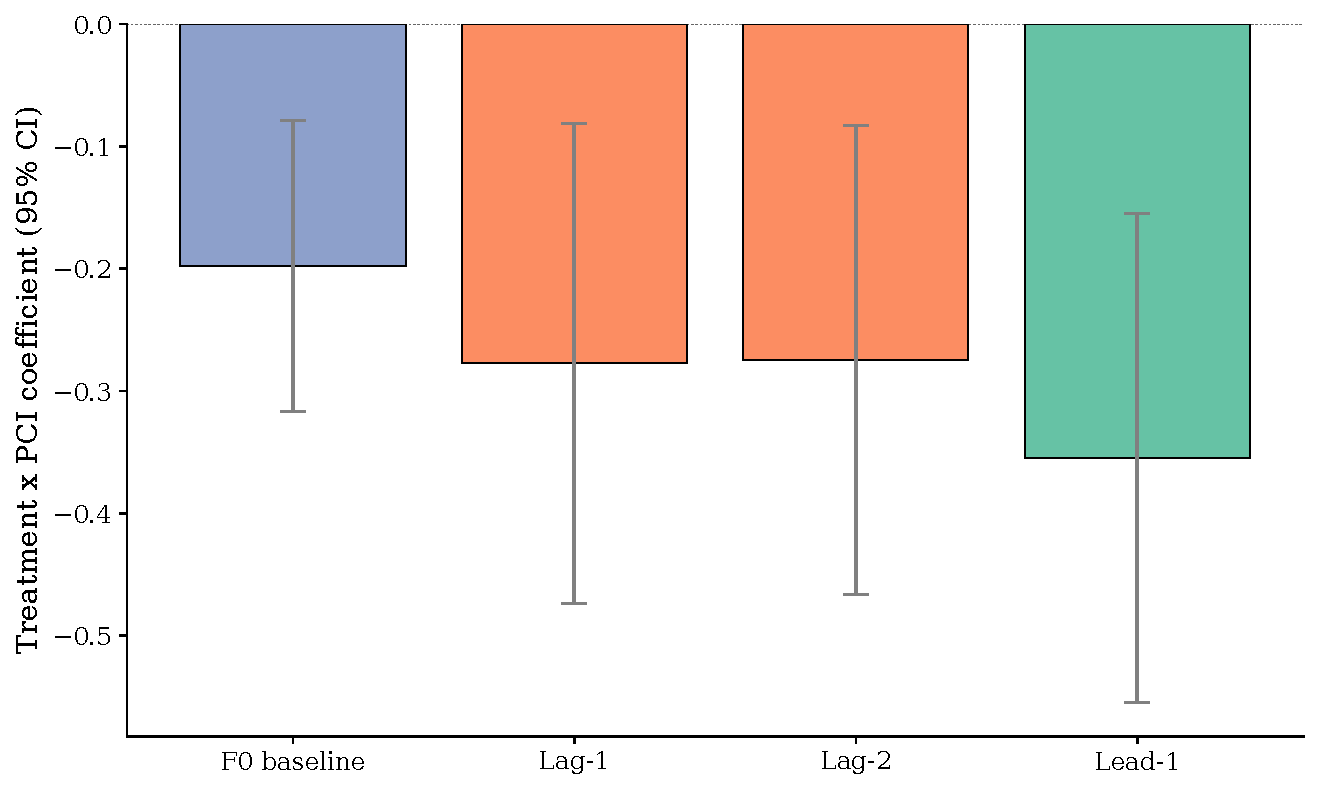
\includegraphics[width=0.7\textwidth]{figures/08_endogeneity/baseline_vs_lead.pdf}
\caption{Baseline vs. Lead De-risking Coefficients by Year}
\label{fig:baseline_lead}
\begin{minipage}{0.9\textwidth}
\footnotesize \textit{Notes.} Year-by-year PPML cross-sections. Baseline uses contemporaneous de-risking; Lead uses $t+1$ de-risking.
\end{minipage}
\end{figure}

\subsection*{A.3 Panel Robustness Specification Curve}

Figure~\ref{fig:spec_panel} presents the specification curve for panel pair-FE estimates across 11 robustness variants.

\begin{figure}[htbp]
\centering
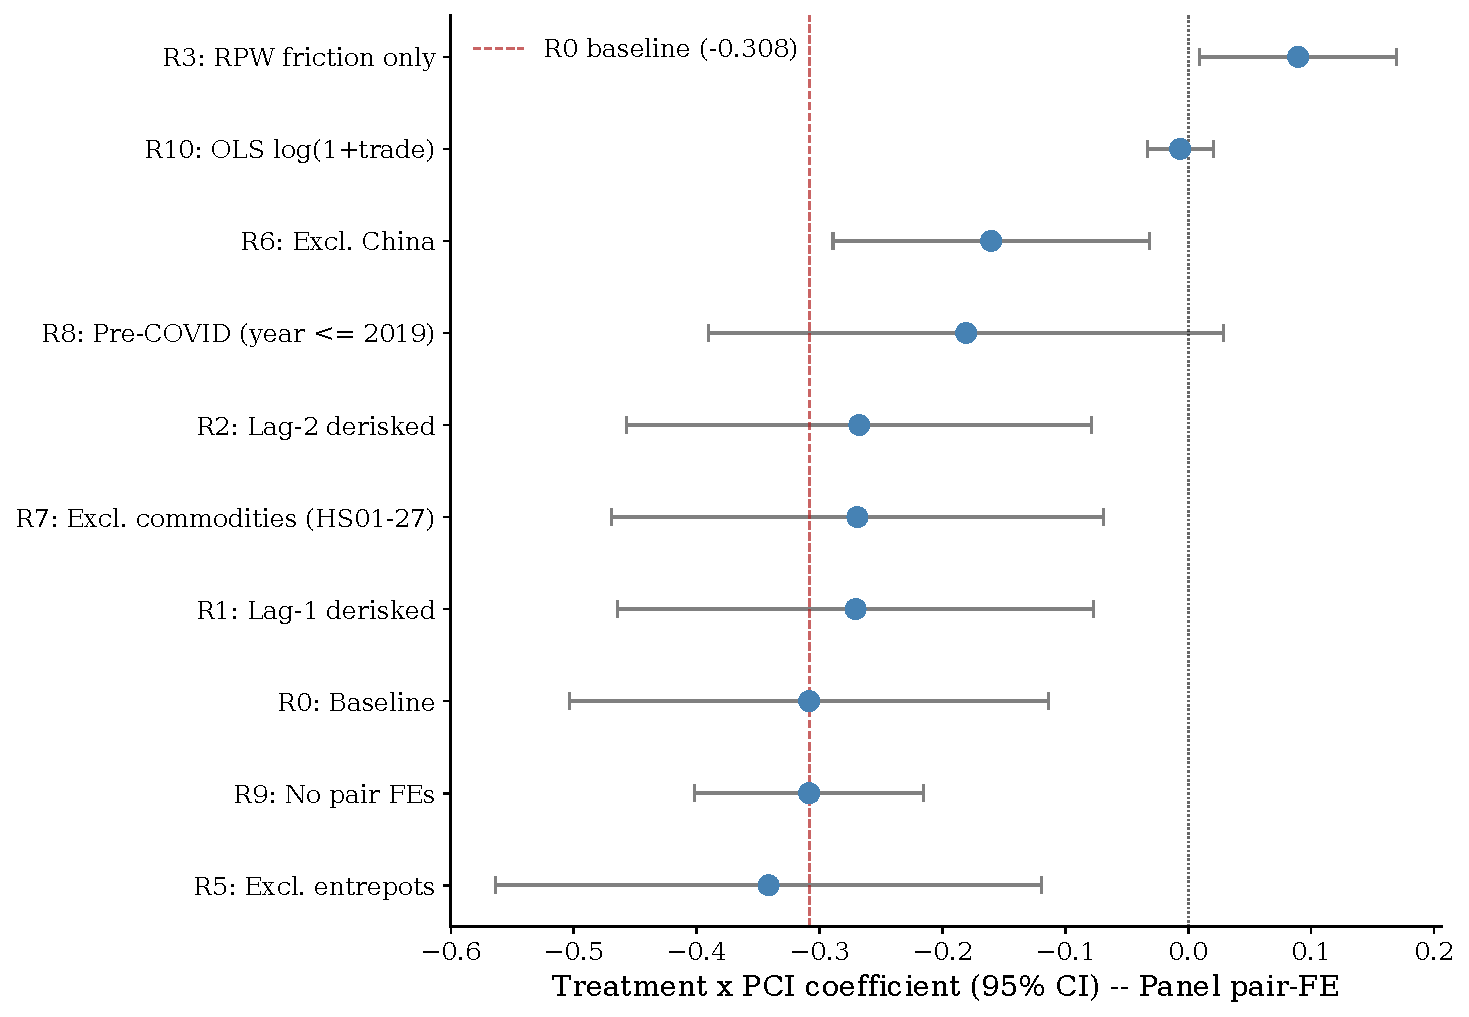
\includegraphics[width=0.85\textwidth]{figures/11_robustness/specification_curve_panel.pdf}
\caption{Specification Curve: Panel Robustness (Pair FE)}
\label{fig:spec_panel}
\begin{minipage}{0.9\textwidth}
\footnotesize \textit{Notes.} Each point represents one specification variant estimated with pair FE on the stratified subsample. Horizontal bars show 95\% confidence intervals.
\end{minipage}
\end{figure}

\subsection*{A.4 Falsification Test Results}

Figure~\ref{fig:falsification} presents the combined falsification panel, showing forest plots of yearly means and panel pair-FE results for all placebo interactions.

\begin{figure}[htbp]
\centering
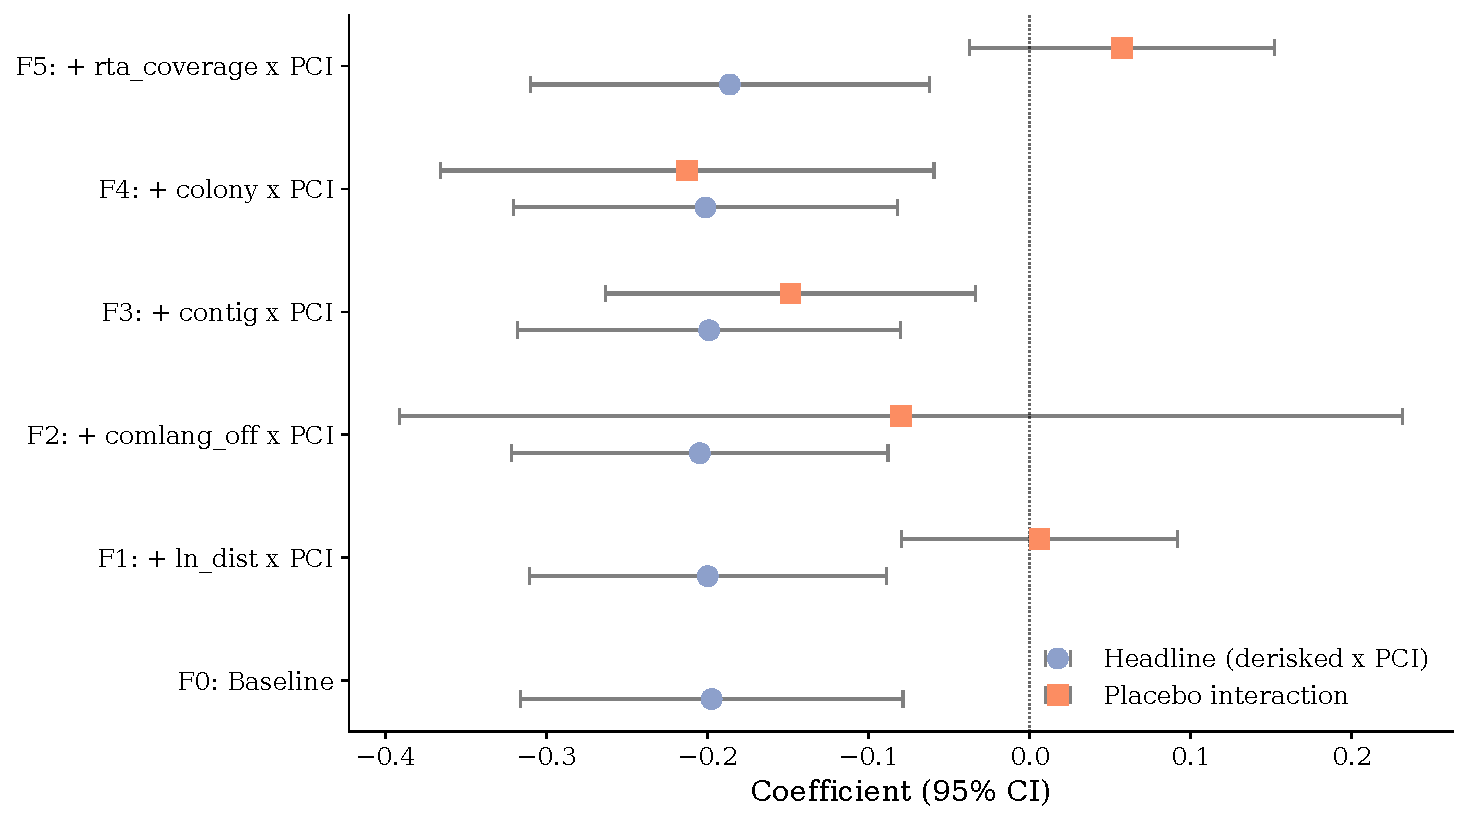
\includegraphics[width=0.85\textwidth]{figures/12_falsification/falsification_panel.pdf}
\caption{Falsification Tests: Forest Plot}
\label{fig:falsification}
\begin{minipage}{0.9\textwidth}
\footnotesize \textit{Notes.} Left panel: yearly mean coefficients with pooled 95\% CI. Right panel: permutation null distribution with baseline coefficient marked.
\end{minipage}
\end{figure}

\subsection*{A.5 De-risking Exposure World Map}

Figure~\ref{fig:derisking_map} maps the number of de-risked bilateral corridors per country.

\begin{figure}[htbp]
\centering
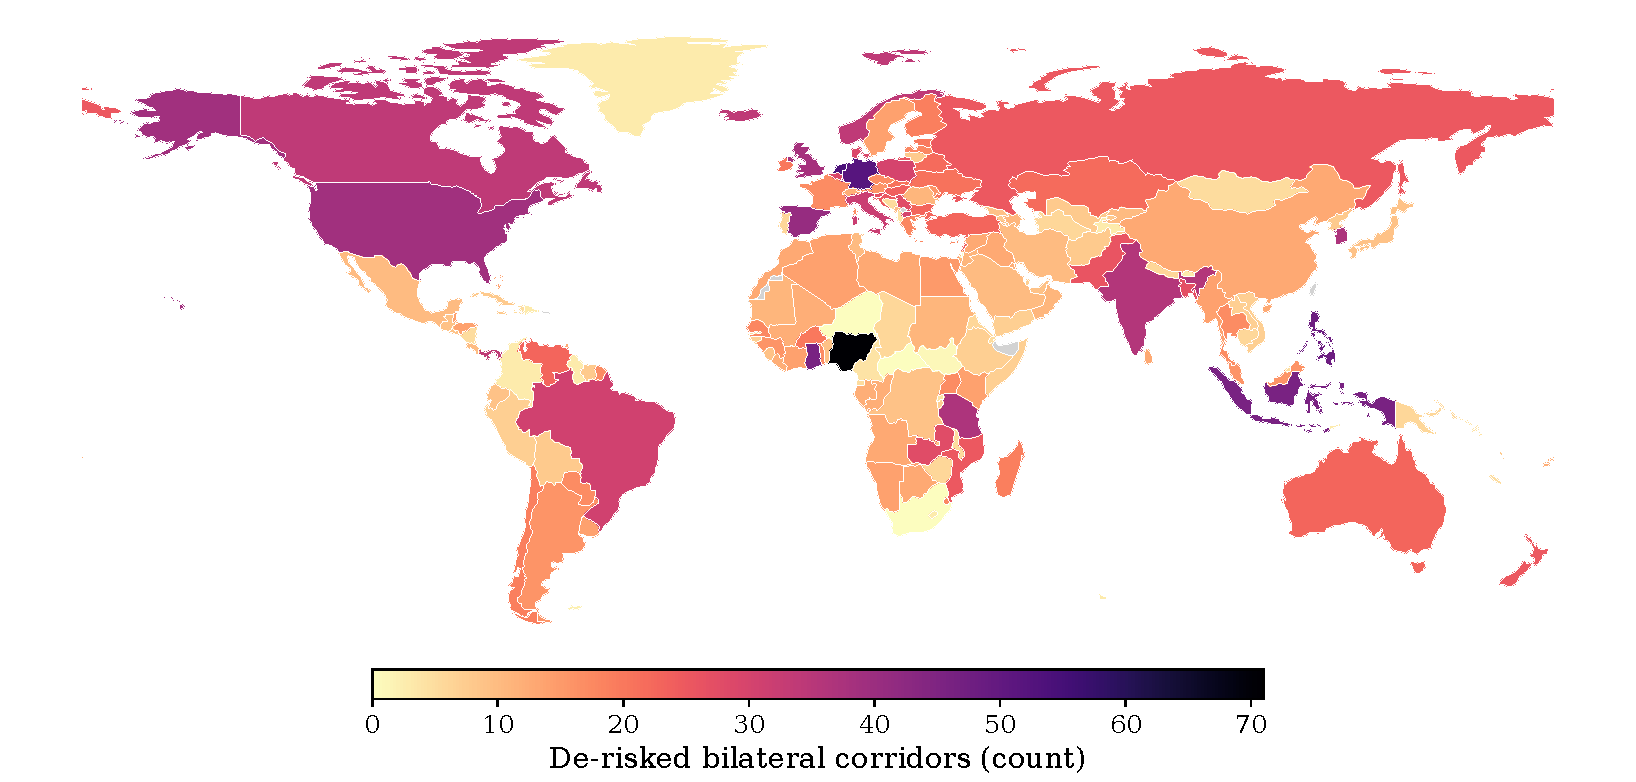
\includegraphics[width=0.95\textwidth]{figures/13_figures/world_derisking_exposure.pdf}
\caption{De-risking Exposure by Country}
\label{fig:derisking_map}
\begin{minipage}{0.9\textwidth}
\footnotesize \textit{Notes.} Country-level count of de-risked bilateral corridors (FDI dropped $>$50\% from the 2015--2017 base), plotted as a choropleth using Natural Earth low-resolution country polygons. Darker shading indicates more de-risked partners; countries with no data shown in light gray.
\end{minipage}
\end{figure}

\subsection*{A.6 SOS Decomposition}

Figure~\ref{fig:sos_decomp} decomposes the SOS into intensive and extensive margin contributions for the top 20 countries.

\begin{figure}[htbp]
\centering
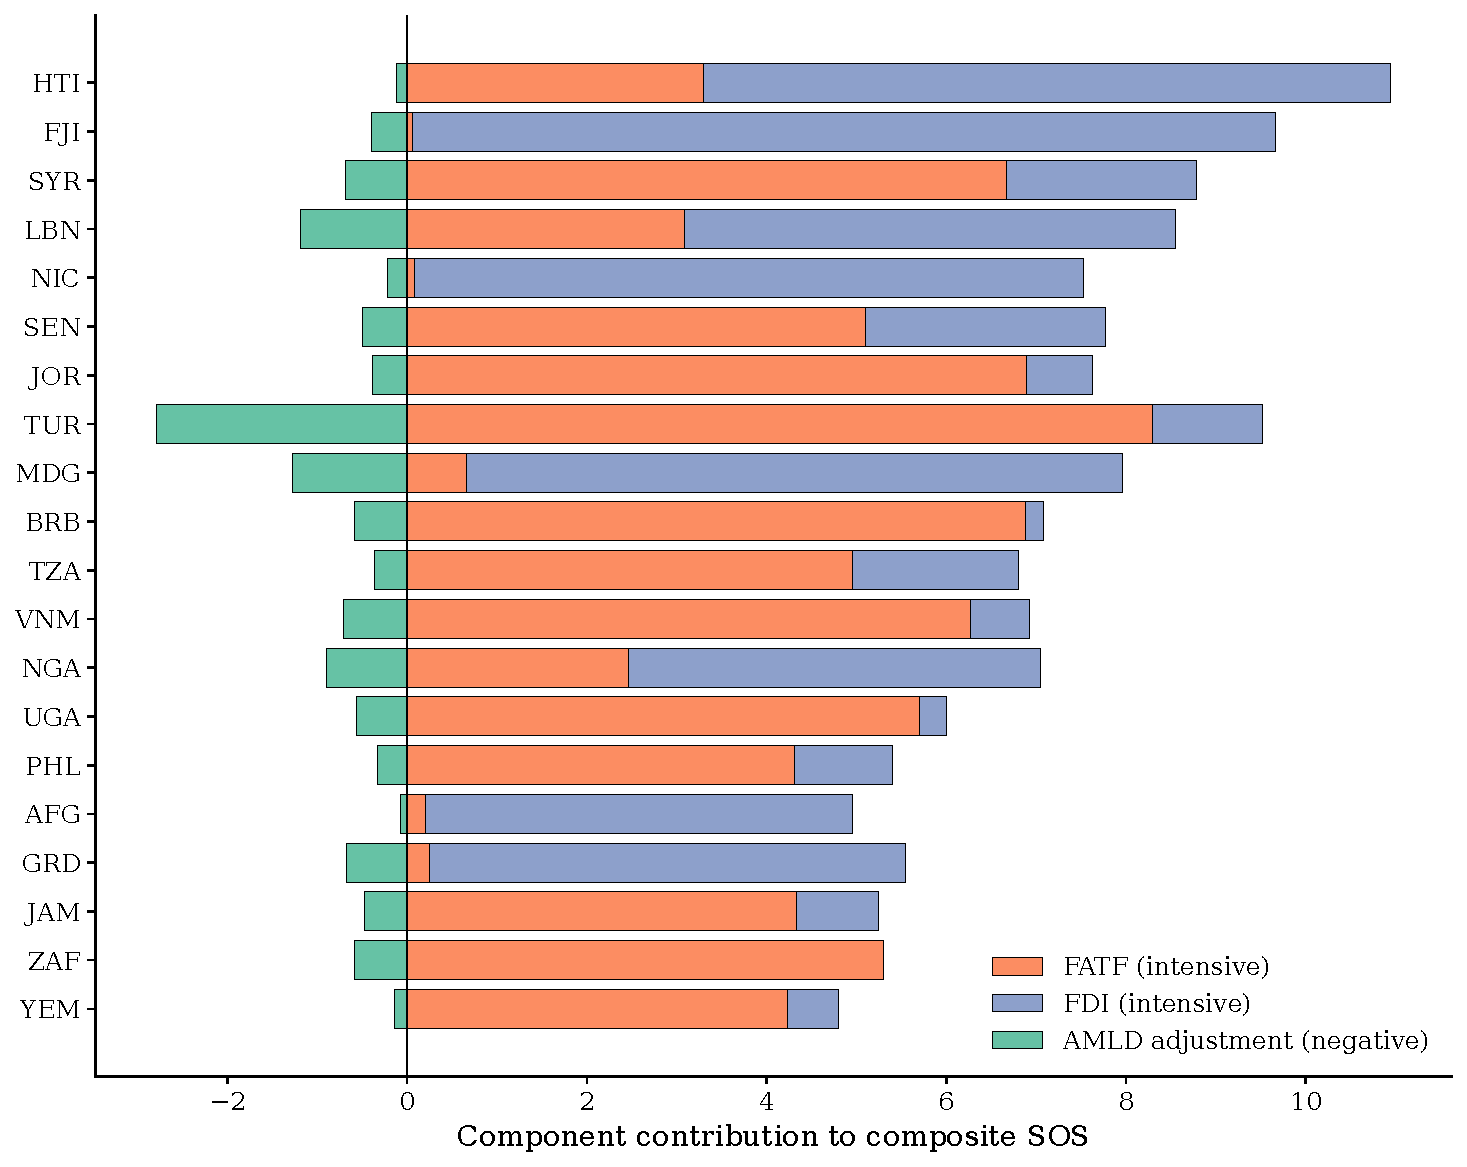
\includegraphics[width=0.8\textwidth]{figures/13_figures/sos_decomposition_top20.pdf}
\caption{SOS Decomposition: Intensive vs. Extensive Margin (Top 20)}
\label{fig:sos_decomp}
\begin{minipage}{0.9\textwidth}
\footnotesize \textit{Notes.} Stacked bar chart. Intensive margin: existing complex trade at risk in de-risked corridors. Extensive margin: unrealized diversification potential.
\end{minipage}
\end{figure}

\subsection*{A.7 SOS Validation: Conditional Scatter}

Figure~\ref{fig:validation} plots the SOS against the Chainalysis Global Crypto Adoption Index, both unconditionally and conditional on GDP per capita.

\begin{figure}[htbp]
\centering
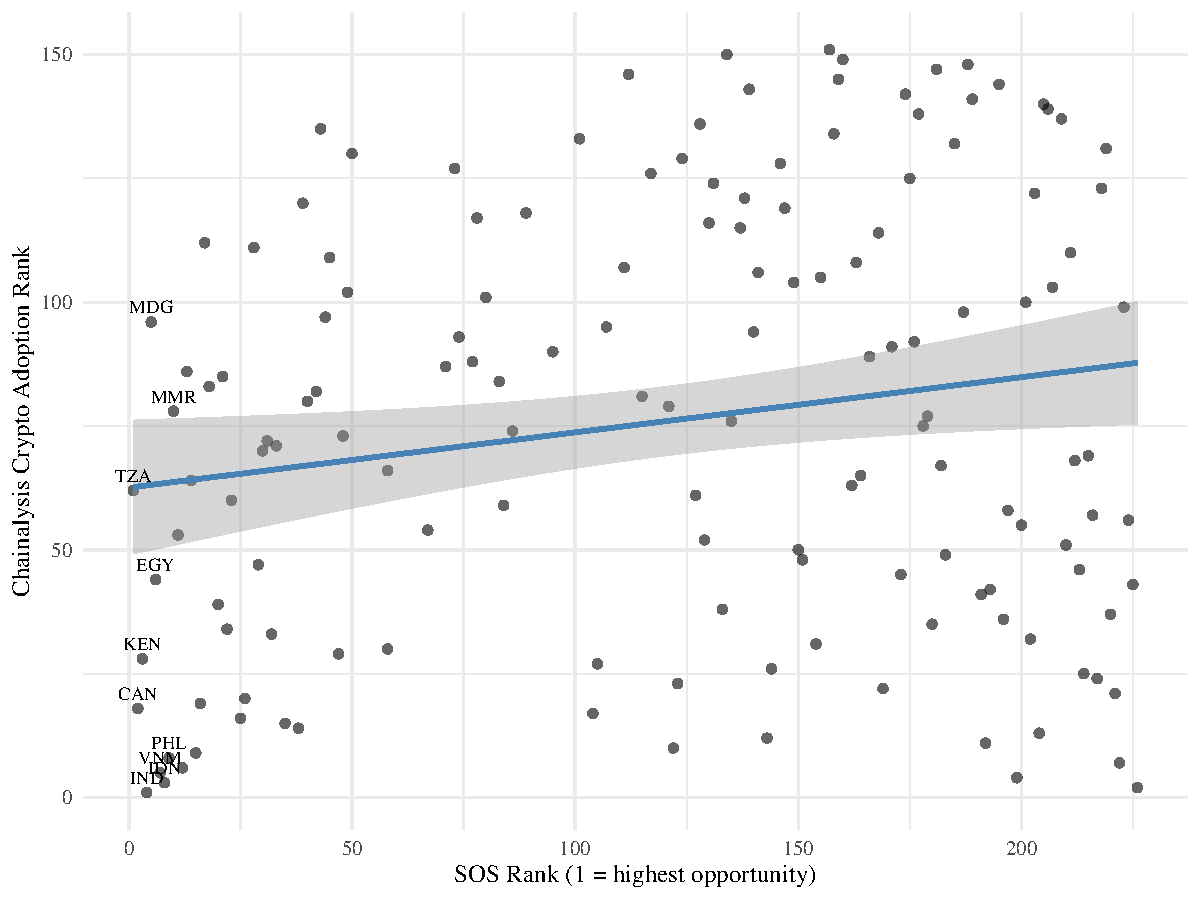
\includegraphics[width=0.7\textwidth]{figures/10_validation/sos_vs_chainalysis.pdf}
\caption{SOS vs. Chainalysis Crypto Adoption Index}
\label{fig:validation}
\begin{minipage}{0.9\textwidth}
\footnotesize \textit{Notes.} Each point is a country ($N = 149$). Unconditional Spearman $\rho = 0.155$; conditional on log GDP per capita, $\rho = 0.126$.
\end{minipage}
\end{figure}


\end{document}
